%!TEX program = lualatex
\DocumentMetadata{testphase=new-or-1}
\documentclass[12pt]{article}
\usepackage{graphicx}
\usepackage{amsmath}
\usepackage{setspace}
\usepackage{microtype}
\usepackage[english]{babel}
\usepackage{csquotes}
\usepackage[stable]{footmisc}
\usepackage[letterpaper, portrait, margin=1in]{geometry}
\usepackage[toc,page]{appendix}
\usepackage{minted}
\usepackage{booktabs}
\usepackage{tabularx}
\usepackage{longtable}
\usepackage{multirow}
\usepackage{lscape}
\usepackage{fancyhdr}
\usepackage[hidelinks]{hyperref}
\pagestyle{fancy}
\usepackage{float}

\usepackage{caption}

% Custom caption setup:
\makeatletter
\DeclareRobustCommand{\caption}{%
  \@ifnextchar[%]
    {\@captionwithopt}
    {\@captionwithoutopt}%
}

\newcommand{\@captionwithopt}[3][]{%
  \if\relax\detokenize{#3}\relax
    % EMPTY caption → number only
    \caption@setopt{#1}%
    \caption@makecaption{\csname fnum@\@captype\endcsname}{}%
  \else
    % NONEMPTY caption → include labelsep (colon)
    \caption@setopt{#1}%
    \caption@makecaption{\csname fnum@\@captype\endcsname}{#3}%
  \fi
}

\newcommand{\@captionwithoutopt}[2]{%
  \@captionwithopt[]{#1}{#2}%
}

\makeatother

% normal caption settings (colon)
\captionsetup{
  labelsep=colon
}


\fancyhf{} % clear headers/footers
\fancyfoot[C]{\thepage} % page number centered bottom
\renewcommand{\headrulewidth}{0pt}
\renewcommand{\footrulewidth}{0pt}

% IMPORTANT: also redefine the 'plain' style used by longtable, etc.
\fancypagestyle{plain}{%
  \fancyhf{}
  \fancyfoot[C]{\thepage}
  \renewcommand{\headrulewidth}{0pt}
  \renewcommand{\footrulewidth}{0pt}
}

\usepackage{fontspec}
\setmainfont{Times New Roman}

% Reduce spurious overfull lines in fully-justified text.
\setlength{\emergencystretch}{1em}
\makeatletter
\renewcommand{\tableofcontents}{\@starttoc{toc}}
\makeatother

\begin{document}
\thispagestyle{empty}
\begingroup  
  \centering
   \large Pandects: Open-Source M\&A Research\\[1em]
  \normalsize Nikita Bogdanov\textsuperscript{*}\\
  \normalsize April 2026\\
\endgroup

\smallskip
\begin{abstract}
Quantitative research on the structure, design, and evolution of M\&A agreements requires high-quality, machine-readable data, and reproducibility considerations counsel that such data be publicly available. Until recently, however, no public corpus of M\&A agreements existed. In 2024, Peter Adelson, Matthew Jennejohn, Julian Nyarko, and Eric Talley took an important first step by identifying the URLs and extracting the text of several provisions for nearly 8,000 definitive M\&A agreements filed on EDGAR from 2000 through 2020. This paper builds on that work by introducing Pandects, the first open-source database of structured M\&A agreements. Pandects uses purpose-built data pipelines, machine learning models, and large language models to convert EDGAR M\&A filings into machine-readable XML; classify agreement sections into a comprehensive taxonomy; and enrich each deal with transaction metadata. Updated monthly and covering agreements back to 2000, Pandects is free and available online, through an API, as a bulk dataset, and via MCP server. This paper describes the infrastructure behind Pandects and demonstrates using Pandects data to update existing research on forum selection clauses.
\end{abstract}

\smallskip
\begingroup
\setstretch{0.9}
\tableofcontents
\endgroup
\vfill
\begingroup
\singlespacing
\noindent{\fontsize{9}{7}\selectfont * J.D. Candidate (2026), New York University School of Law. nmbogdan@alumni.stanford.edu. Professor Emiliano Catan actively advised this project from the beginning. The Jacobson Leadership Program in Law and Business provided all startup funding. We are also grateful to professor Chris Sprigman. Jack Cushman at Harvard Law's Library Innovation Lab provided early advice. Josh Carty provided early technical assistance. This project would not have gotten off the ground without the prior work of Peter Adelson, Matthew Jennejohn, Julian Nyarko, and Eric Talley. Finally, this project was supported in part through NYU IT High Performance Computing resources, services, and staff expertise. \emph{AI disclaimer: LLMs wrote the vast majority of the code. While we used LLMs to generate this paper's tables and figures, to the best of our knowledge we have authored all substantive content ourselves.}}
\endgroup
\newpage
\doublespacing

\section{Introduction}
Data is the \emph{sine qua non} of quantitative research. Yet until recently, quantitative researchers interested in M\&A lacked a definitive dataset on which to rely. In 2024, Peter Adelson, Matthew Jennejohn, Julian Nyarko, and Eric Talley took an important first step toward closing this gap when they released their corpus of definitive merger agreements (“DMA Corpus”).\footnote{Peter Adelson et al., \emph{Introducing a New Corpus of Definitive M\&A Agreements, 2000-2020} (Columbia Law and Economics Working Paper No. 4731282), \url{https://papers.ssrn.com/sol3/papers.cfm?abstract_id=4731282}.} Adelson et al. describe their motivation as follows:

\begingroup
\singlespacing
\begin{quote}
It remains difficult for empirically minded contract scholars to access clean, readable corpora of relevant contractual texts. Those who have built such corpora have at times been reluctant to share them. On other occasions, authors report that they are prohibited from doing so by restrictive licensing practices. These constraints have placed a barrier to entry within the field of empirical contracts that makes it difficult to accomplish reproducibility, a core condition for the advancement of the field.\footnote{\emph{Id.} at 2.}
\end{quote}
\endgroup
\vspace{-1em}

Several points are worth highlighting. First, there are at least three—and likely many more—commercial solutions that enable exactly the kinds of analyses the DMA Corpus aims to facilitate.\footnote{Deal Point Data is one prominent such solution. \url{https://www.dealpointdata.com/}.}  As Adelson et al. report, however, these solutions often subject their users to restrictive licenses, making it challenging, if not impossible, for academics to release the data upon which their studies rely. Second, data consistency across quantitative research projects enhances research integrity. The absence of a definitive corpus leads researchers to duplicate unglamorous data processing work and complicates comparisons across studies. Finally, though Adelson et al. do not discuss this point, quantitative researchers perennially complain about data freshness: researchers may put together a corpus spanning the most recent 5, 10, or 20 years, but without a mechanism or plan to update that corpus, the corpus soon becomes stale and loses research relevance.

The DMA Corpus takes an important first step toward creating a public database of M\&A agreements. It collects 7,929 definitive merger agreements filed with the SEC between 2000 and 2020, and in addition to identifying the EDGAR URL for each, surfaces the text of MeToo provisions, pandemic MAE carveouts, and several other provisions. But, as significant a development as the DMA Corpus is, it leaves substantial room for extension. First, at least in its current state, the DMA Corpus is frozen in time, collecting definitive M\&A agreements through 2020 only. Second, the DMA Corpus surfaces the text of only a limited number of clauses; researchers interested in provisions beyond that relatively narrow set must process raw agreement text on their own. Finally, the DMA Corpus does not include any substantial transaction metadata outside of target, acquirer, and year; for instance, the corpus does not provide transaction value, consideration type, party industries, and other similar data.

The Pandects\footnote{The name derives from the Pandects, Roman Emperor Justinian's 6th-century compendium that distilled centuries of legal wisdom into a single, authoritative digest.} project builds on the DMA Corpus to create the first open-source database of structured M\&A agreements: we extend the DMA Corpus up through the present on a continuous basis, roughly every four weeks; create XML representations of each agreement; classify agreement sections into a comprehensive taxonomy; and enrich agreements with metadata. In addition to developing and maintaining the core dataset, the Pandects project goes out of its way to make this dataset easily accessible. The project is currently hosted online at pandects.org, where researchers can find the latest database version for bulk download or access it programmatically via API; we have also developed an MCP server, to allow LLMs to connect to and query the database.\footnote{MCP, or Model Context Protocol, is an open-source standard for connecting generative AI applications such as LLMs to external systems such as databases. \url{https://modelcontextprotocol.io/}. The Pandects MCP server is available free of charge, but requires creating an account with Pandects.} To aid adoption, we have put together a series of example Jupyter Notebooks,\footnote{\url{https://github.com/PlatosTwin/pandects-app/tree/main/examples}.} which walk through pulling data via the API; we have also invested in a comprehensive technical documentation microsite.\footnote{\url{https://docs.pandects.org/}.} Finally, the project encourages users to flag errors and submit corrections, so as to crowdsource corpus data quality improvements.\footnote{See \autoref{app:flag-agreements}.} The project is fully open source, with all code available under a GNU GPLv3 license,\footnote{\url{https://www.gnu.org/licenses/gpl-3.0.en.html}.} while all data is available under v1 of the Open Database License.\footnote{\url{https://opendatacommons.org/licenses/odbl/1-0/}.} The Harvard Caselaw Access Project has served as an important guide.\footnote{The Harvard Caselaw Access Project digitized and made publicly available the entirety of United States case law in the Harvard Law Library up through 2018. \url{https://case.law/}.}

In \autoref{sec:infrastructure-data}, we outline the technical infrastructure that powers Pandects. In \autoref{sec:putting-pandects-to-work}, we demonstrate how researchers might use Pandects data to update existing research on forum selection clauses.

\section{Infrastructure and Data}\label{sec:infrastructure-data}

\subsection{Infrastructure}\label{sec:infrastructure}
At the heart of Pandects is an ETL pipeline that employs purpose-built machine learning models to ingest agreements, segment them into pages, tag articles and sections, generate XML, classify sections within a taxonomy, and add metadata. What follows is a high-level overview of the pipeline’s components; because Pandects data updates every four weeks, each of these components runs, in sequence, on a roughly monthly basis. We have included similar detail online, under Data \textgreater{} Sources \& Methods,\footnote{\url{https://pandects.org/sources-methods}.} which, unlike this paper, will always have the latest information.\footnote{All model code is available on GitHub: \url{https://github.com/PlatosTwin/pandects-app/tree/main/etl/src/etl/models}.}

\subsubsection{Data Ingestion}\label{sec:data-ingestion}
For agreements from 2000 through 2020, we simply ingest the agreements in the DMA Corpus, which is a one-time task. To identify agreements from 2021 through the present, however, we develop a purpose-built exhibit classifier model. The exhibit model takes as inputs filings from the SEC’s EDGAR database, and for each filing, outputs the probability that that filing represents a definitive merger agreement. To identify filings, we scan the SEC's daily index files, identify all filings that match target form types (all forms except for S-8 and ABS-EE), filter filings by scanning for keywords indicating ``Material Definitive Agreement'' entries, scrape each filing's index page to extract Exhibit 2 and 10 links, fetch and render the exhibit content as text, and use the Exhibit Model to classify candidates. Note that, unlike the DMA Corpus, we do \emph{not} scan Exhibit 99 filings; however, given the distribution of Exhibit 99 filings in the DMA Corpus, we do not expect there to be a material number of relevant agreements filed under Exhibit 99.\footnote{Of the 7,929 agreements in the DMA Corpus, 264 (3.3\%) derive from Exhibit 99 filings. Only 54 of these agreements (20\% of 264, 0.68\% of 7,929) were filed between 2010 and 2020, with the remaining 210 filed between 2000 and 2009. What's more, 19 (7\% of 264, 0.24\% of 7,929) derive from agreements filed between 2016 and 2020, for an average of 3.8 per year for the last five years available in the DMA Corpus, an immaterial number.}

\underline{\smash{Architecture}}: The exhibit model is a tuned logistic-regression classifier over three feature blocks: (1) document-level features such as opening title phrases, hard-negative phrase counts, document length, and M\&A keyword density; (2) hashed word- and character-level TF-IDF features; and (3) similarity features capturing max, mean, and median cosine similarity to the training agreement corpus. We also apply a minimum-length hard-negative rule and use a tuned decision threshold of 0.96.

\underline{\smash{Training corpus}}: We begin with 8,889 labeled exhibits: 7,919 positives—all from the DMA Corpus—and 970 negatives, which we draw from SEC filings under Exhibits 2 and 10.\footnote{We were unable to access the URLs for 10 of the 7,929 agreements.} After dropping 23 short positive exhibits to align the training set with the model's minimum-length hard-negative rule, we split the remaining 8,866 exhibits into 6,206 training exhibits, 886 validation exhibits, and 1,774 holdout test exhibits, stratified on class.

\underline{\smash{Performance}}: We evaluate the Exhibit Model as a binary classifier, where the positive class indicates that an exhibit is a definitive merger agreement. We report accuracy, precision, recall, and \(F_1\), along with ROC AUC. Because the model is used as a high-precision filter before downstream processing, we tune the decision threshold (0.96) to limit false positives, subject to the ad hoc constraint of keeping recall at or above 97\%.

It is worth highlighting that the class distributions we use in training and evaluation are not representative of the class distribution in practice, because in practice, the Exhibit Model sees primarily irrelevant filings, which is one reason we tune for higher precision. A further caveat is that the metrics we report here are for the Exhibit Model itself, not for the end-to-end staging pipeline, which uses various deterministic rules to pre-screen filings before they even make it to the Exhibit Model. That said, in a random sample of 699 non-Exhibit 99 agreements from the DMA Corpus from 2015 onwards, 694 agreements (99.3\%) made it through pre-screening, so it is the Exhibit Model that is doing the important selection work, not earlier deterministic filtering.\footnote{Filings from prior to 2015 are screened out at higher rates, but are not representative of the filings our screening logic will see.}

\begin{table}[H]
\centering
\caption{Exhibit Model overall holdout test metrics.}
\label{tab:exhibit-overall}
\begin{tabular}{rrrrr}
\toprule
Accuracy & Precision & Recall & \(F_1\) & ROC AUC \\
\midrule
97.24\% & 99.74\% & 97.15\% & 98.43\% & 99.61\% \\
\bottomrule
\end{tabular}
\end{table}

\begin{table}[H]
\centering
\caption{Exhibit Model confusion matrix (holdout test).}
\label{tab:exhibit-cm}
\begin{tabular}{lrr}
\toprule
 & Pred.\ negative & Pred.\ positive \\
\midrule
Actual negative & 190 & 4 \\
Actual positive & 45 & 1535 \\
\bottomrule
\end{tabular}
\end{table}

\begin{table}[H]
\centering
\caption{Exhibit Model per-class metrics (holdout test).}
\label{tab:exhibit-per-class}
\begin{tabular}{lrrrr}
\toprule
Class & Precision & Recall & \(F_1\) & Support \\
\midrule
Negative & 80.85\% & 97.94\% & 88.58\% & 194 \\
Positive & 99.74\% & 97.15\% & 98.43\% & 1{,}580 \\
\bottomrule
\end{tabular}
\end{table}

\subsubsection{Text Processing}\label{sec:text-processing}
For every staged agreement, we visit EDGAR, download the agreement’s raw text or HTML, clean and standardize the text, split the agreement into individual pages, and then use a purpose-built classifier model to classify pages into one of five classes (front matter, table of contents, body, signature, back matter). While classifying pages in this manner adds to the pipeline's overall complexity, the tradeoffs are worth it: sending only body pages through our Named Entity Recognition model eliminates the possibility of erroneous tags outside of the body section.

\underline{\smash{Architecture}}: The page classifier model is a document-level monotonic CRF. Each page is featurized with positional, structural, and lexical signals, including relative page position, heading patterns, TOC dots, signature and witness markers, annex and appendix anchors, and compact TF-IDF word features. A constrained CRF then predicts the full page sequence in one pass while enforcing monotonic transitions through \texttt{front\_matter}, \texttt{toc}, \texttt{body}, \texttt{sig}, and \texttt{back\_matter}.

\underline{\smash{Training corpus}}: We train the page CRF on 67,596 manually labeled pages across 673 agreements. We split the corpus by agreement, not by page, so that pages from the same agreement never land in both fit and holdout sets. The fixed manifest contains 41,394 training pages across 404 agreements, 13,306 validation pages across 139 agreements, and 12,896 holdout test pages across 130 agreements, stratified by announcement year and agreement type.

\underline{\smash{Performance}}: We evaluate the Page Classifier using standard multiclass classification metrics. We report overall accuracy and macro-averaged precision, recall, and \(F_1\) across the five page classes. Because the classifier is constrained to monotonic transitions (from \texttt{front\_matter} through \texttt{back\_matter}), most errors arise at class boundaries—especially at the \texttt{body}/\texttt{back\_matter} boundary, where schedules and annexes vary substantially across agreements.

\begin{table}[H]
\centering
\caption{Page Classifier overall metrics (validation vs.\ holdout test).}
\label{tab:page-crf-overall}
\begin{tabular}{llrrrr}
\toprule
Split & Run & Accuracy & Precision & Recall & \(F_1\) \\
\midrule
Validation & Tuned CRF & 97.68\% & 96.63\% & 96.84\% & 96.67\% \\
Test & Final CRF & 96.00\% & 93.94\% & 96.31\% & 95.08\% \\
\bottomrule
\end{tabular}
\end{table}

\begin{table}[H]
\centering
\caption{Page Classifier per-class metrics (validation: tuned CRF).}
\label{tab:page-crf-per-class-val}
\begin{tabular}{lrrrr}
\toprule
Class & Precision & Recall & \(F_1\) & Support \\
\midrule
\texttt{front\_matter} & 98.06\% & 99.35\% & 98.70\% & 153 \\
\texttt{toc} & 99.25\% & 99.07\% & 99.16\% & 536 \\
\texttt{body} & 99.68\% & 97.51\% & 98.59\% & 10{,}040 \\
\texttt{sig} & 96.38\% & 89.50\% & 92.81\% & 238 \\
\texttt{back\_matter} & 89.78\% & 98.80\% & 94.08\% & 2{,}339 \\
\bottomrule
\end{tabular}
\end{table}

\begin{table}[H]
\centering
\caption{Page Classifier per-class metrics (holdout test: final CRF).}
\label{tab:page-crf-per-class-test}
\begin{tabular}{lrrrr}
\toprule
Class & Precision & Recall & \(F_1\) & Support \\
\midrule
\texttt{front\_matter} & 96.93\% & 96.93\% & 96.93\% & 163 \\
\texttt{toc} & 98.33\% & 99.16\% & 98.74\% & 476 \\
\texttt{body} & 98.15\% & 96.58\% & 97.36\% & 9{,}324 \\
\texttt{sig} & 86.98\% & 95.43\% & 91.01\% & 175 \\
\texttt{back\_matter} & 89.33\% & 93.47\% & 91.35\% & 2{,}758 \\
\bottomrule
\end{tabular}
\end{table}

\begingroup
\small
\begin{table}[H]
\centering
\caption{Page Classifier confusion matrix (validation: tuned CRF).}
\label{tab:page-crf-cm-val}
\begin{tabular}{lrrrrr}
\toprule
 & FM & TOC & BDY & SIG & BM \\
\midrule
FM  & 152 & 1 & 0 & 0 & 0 \\
TOC & 3 & 531 & 2 & 0 & 0 \\
BDY & 0 & 3 & 9790 & 3 & 244 \\
SIG & 0 & 0 & 6 & 213 & 19 \\
BM  & 0 & 0 & 23 & 5 & 2311 \\
\bottomrule
\end{tabular}
\end{table}
\endgroup

\begingroup
\small
\begin{table}[H]
\centering
\caption{Page Classifier confusion matrix (holdout test: final CRF).}
\label{tab:page-crf-cm-test}
\begin{tabular}{lrrrrr}
\toprule
 & FM & TOC & BDY & SIG & BM \\
\midrule
FM  & 158 & 3 & 2 & 0 & 0 \\
TOC & 4 & 472 & 0 & 0 & 0 \\
BDY & 1 & 5 & 9005 & 12 & 301 \\
SIG & 0 & 0 & 1 & 167 & 7 \\
BM  & 0 & 0 & 167 & 13 & 2578 \\
\bottomrule
\end{tabular}
\end{table}
\endgroup

\subsubsection{Article and Section Tagging}\label{sec:article-section-tagging}
This pipeline stage takes as inputs individual pages from M\&A agreements and uses a purpose-built Named Entity Recognition (NER) model to label article and section headings, as well as page numbers.

\underline{\smash{Architecture}}: The NER model fine-tunes ModernBERT-base\footnote{\url{https://huggingface.co/answerdotai/ModernBERT-base}.} for token-level labeling of Article, Section, and Page entities. The current production recipe uses an independent decoder, a lightweight auxiliary boundary head for Article and Section start/end detection, focal token loss, preserved input casing, and boundary-mix sampling over fixed-length token windows. At inference time, overlapping windows are stitched by averaging logits and then lightly repaired into valid BIO-style sequences before tags are rendered back into the page text. We use BIOE tags for Articles and Sections, plus BIOES-style tags for Pages.

\underline{\smash{Training corpus}}: We used gpt-5.1 to create a page-level structural tagging corpus of 11,022 agreement pages (body pages only).\footnote{See \autoref{app:training-data-prompt} for the prompt we used.} Of these, 8,157 derive from 115 agreements, which we tagged in full; we selected an additional 2,865 at random to include more examples of Article tags. Among these 11,022 pages, 7,451 have at least one tagged Section, 2,487 have at least one tagged Article, and 3,547 are clean negatives. (Note that many pages have both Article and Section tags.) Across this set, we evaluated a small sample manually, based on which we programmatically normalized whitespace treatment, to ensure that tags did not enclose whitespace at the start or end of titles; we also validated that all tagged text compiled into a valid agreement structure, using the same hard validation rules we deploy in the XML construction and validation step. Thereafter, we augmented the corpus with another 35,038 pages from 443 agreements that an earlier version of the Tagging Model labeled and that passed the same XML validator, for a total corpus of 46,060 pages from 754 agreements. We split the corpus by agreement, not by page, so that pages from the same agreement never land in both train and holdout sets. The fixed manifest contains 39,416 train pages across 664 agreements, 3,335 validation pages across 45 agreements, and 3,309 test pages across 45 agreements; as with the preceding models, the test split is reserved for final evaluation only. All 2,865 Article-oversampled pages remain train-only, so that entity distributions in the validation and test splits approximate those the model will see in practice.

\underline{\smash{Performance}}: We evaluate the Tagging Model using standard entity-level precision, recall, and \(F_1\), micro-averaged over all predicted entity spans. We report two scoring modes. \emph{Strict} scoring counts a prediction as correct only if the predicted span \emph{exactly} matches the gold span boundaries and entity type; \emph{lenient} scoring counts a prediction as correct if it matches the correct entity type and overlaps the gold span. In addition to span-level metrics, we also report boundary \(F_1\) by tag position (\texttt{B}, \texttt{I}, \texttt{E}, and \texttt{S}) to highlight where errors concentrate.

While the model performs exceptionally well at the level of pages, it is important to emphasize that page-level performance does not translate directly into agreement-level performance. As a concrete example, with 10,641 agreements and extrapolating from the observed average of roughly 97.5 sections per agreement, we would expect approximately 1,037,797 sections. Given our model's precision and recall,\footnote{Total errors \(= \mathrm{FP} + \mathrm{FN}\), where \(\mathrm{TP} = R \cdot N\), \(\mathrm{FN} = (1 - R) \cdot N\), and \(\mathrm{FP} = \mathrm{TP} \cdot (1/P - 1)\), with \(N\) the number of true sections and \(P\) and \(R\) strict precision and recall, respectively.} that translates to roughly 3,011 errors—either false positives or false negatives. At worst, with one error per agreement, these 3,011 errors would invalidate 3,011 agreements, for an agreement-level success rate of 72\%. At best, with 97 errors per agreement, they would concentrate in 32 agreements for an agreement-level success rate of effectively 100\%. In practice, we observe a raw success rate around 88\%, which we then drive higher with various repair logic, outlined further below.

\begin{table}[H]
\centering
\caption{Tagging Model entity-level micro metrics (overall).}
\label{tab:tagging-overall-micro}
\begin{tabular}{lrrr}
\toprule
Scoring mode & Precision & Recall & \(F_1\) \\
\midrule
Strict  & 99.82\% & 99.89\% & 99.86\% \\
Lenient & 99.93\% & 100.00\% & 99.96\% \\
\bottomrule
\end{tabular}
\end{table}

\begin{table}[H]
\centering
\caption{Tagging Model span metrics by entity type.}
\label{tab:tagging-per-entity}
\begin{tabular}{llrrr}
\toprule
Entity & Scoring mode & Precision & Recall & \(F_1\) \\
\midrule
\multirow{2}{*}{Article} & Strict  & 100.00\% & 100.00\% & 100.00\% \\
                        & Lenient & 100.00\% & 100.00\% & 100.00\% \\
\midrule
\multirow{2}{*}{Section} & Strict  & 99.83\% & 99.87\% & 99.85\% \\
                         & Lenient & 99.96\% & 100.00\% & 99.98\% \\
\midrule
\multirow{2}{*}{Page} & Strict  & 99.79\% & 99.91\% & 99.85\% \\
                     & Lenient & 99.88\% & 100.00\% & 99.94\% \\
\bottomrule
\end{tabular}
\end{table}

\begin{table}[H]
\centering
\caption{Tagging Model boundary \(F_1\) by tag position.}
\label{tab:tagging-boundary-f1}
\begin{tabular}{lrrrr}
\toprule
Entity & \texttt{B} & \texttt{I} & \texttt{E} & \texttt{S} \\
\midrule
Article & 100.00\% & 100.00\% & 100.00\% & N/A \\
Section & 99.98\% & 99.94\% & 99.87\% & N/A \\
Page    & 99.72\% & 99.72\% & 99.72\% & 99.87\% \\
\bottomrule
\end{tabular}
\end{table}

\subsubsection{XML and Section Construction}\label{sec:xml-section-construction}
This pipeline stage consumes tagged agreements, turns them into structured XML documents, validates each document using a series of deterministic rules and then gpt-5.4-mini,\footnote{See \autoref{app:xml-validation-prompt} for the validation prompt we use.} and finally splits each document into individual sections and inserts those sections into a dedicated table in the Pandects database. Among paginated agreements, the first-pass validation rate—the proportion of ingested agreements for which the pipeline produces valid XML—is roughly 92\%.

Those agreements that do not make it past XML validation enter a parallel repair and validation flow, where we ask gpt-5.4-mini to tag from scratch each page with a suspected tagging error, and then additionally ask gpt-5.4 whether our NER model's tags are correct and it is the agreement text itself that is corrupted.\footnote{For instance, one agreement progresses straight from 4.10 to 4.12. \url{https://www.sec.gov/Archives/edgar/data/862861/000095017023013095/jan-ex10_95.htm}. Another has two sections labeled 12.1. \url{https://www.sec.gov/Archives/edgar/data/1863181/000114036123012443/ny20008306x2_ex2-1.htm}. Such examples unfortunately abound.}

\subsubsection{Taxonomy Classification}\label{sec:taxonomy-classification}
This pipeline stage assigns each section to one or more classes in the Pandects taxonomy. Initially, we intended to train a multiclass classification model to taxonomize; after some experimentation, however, we determined that using gpt-5.4-mini—or gpt-5.4, for more complicated batches—was substantially more effective while not being cost-prohibitive. As of this writing, then, we taxonomize sections using a mix of gpt-5.4-mini and gpt-5.4. That said, we are actively experimenting with DeepSeek-V4-Pro, run via the NYU HPC cluster and SGLang.\footnote{\url{https://www.sglang.io/}.}

For each section, the LLM sees the title for that section and the title for that section's parent article, as well as the section and parent article titles for the preceding and following sections.\footnote{\url{https://pandects.org/taxonomy}. See \autoref{app:taxonomy-prompt} for the classification prompt we use.} Critically, this means that the LLM \emph{never} sees the actual section text. Additionally, this means that we are presently unable to capture definitions, which typically nest under a ``Definitions'' article as plain text—another important limitation. Finally, it is worth noting that while we are reasonably confident in the performance of gpt-5.4-mini and gpt-5.4, based on spot-checks, as of this writing we do not have any mechanism for validating taxonomy assignments at scale.

For the foregoing reasons, we consider the taxonomy to be largely provisional and subject to change based on input from the research community. We welcome feedback on the taxonomy, as well as collaboration on the development of more granular methods of taxonomizing—e.g., moving to the clause level instead of working at the level of sections alone.

\subsubsection{Metadata Enrichment}\label{sec:metadata-enrichment}
This final pipeline stage uses OpenAI’s web search tool in combination with gpt-5.4-mini—or, when metadata comes back as null, gpt-5.4—to find for each underlying transaction the consideration type, deal size, and various details about the parties, collected in \autoref{app:transaction-metadata}.\footnote{See \autoref{app:offline-metadata-prompt} and \autoref{app:web-search-metadata-prompt} for the prompts we use.} This agreement-level metadata enables transaction filtering. While we have good reason to believe that this data is accurate, especially for large and well-publicized transactions, and while we have certain checks in place, described in the appendix, we cannot guarantee the accuracy of our metadata. That said, we have infrastructure in place to be able to flag agreements as ``verified'' once they have been reviewed manually, and it is our hope that we will be able to crowdsource verification for at least the most significant deals.\footnote{In \autoref{app:flag-agreements} we show the current user interface for the converse of verification: identifying agreements with data \emph{issues}.}

\subsubsection{Update Frequency}\label{sec:update-frequency}
The entire pipeline runs (roughly) once every four weeks with a look-back delay of one week, to allow for media coverage of the deal to appear online. Each pipeline run updates the database accessible online, such that data available via bulk download and API, and in the UI, is at most five weeks old at any point in time (plus an allowance of a day or so for processing time).

\subsection{Data}\label{sec:data}

As of April 10, 2026, Pandects has ingested 10,641 agreements (928,891 pages) filed between January 1, 2000 and April 10, 2026. Our pipelines have processed 9,465 of them, resulting in 923,104 sections. 469 agreements are not paginated; because our pipelines require pagination, any non-paginated agreements drop out.\footnote{Non-pagination is an issue largely for agreements filed in and before 2007, which account for 321 of the 469 (68\%) non-paginated agreements. Between 2020 and 2026, a mere 21 agreements lacked pagination.} Another 707 require additional validation.\footnote{55 (0.5\% of total) are difficult to fit into the 5-class page taxonomy we establish above. 652 (6.1\% of total) are blocked for XML validation due to, for example, missing sections (e.g., progressing from 5.6 to 5.8) or beginning with a section rather than an article.} Metadata coverage varies by metadata field, but in general, core metadata fields such as consideration type, acquirer and target type, acquirer and target industry, and deal purpose have coverage of at least 97\% across processed agreements.\footnote{The Agreement Index page online will always provide the most up-to-date metadata coverage statistics. \url{https://pandects.org/agreement-index}.} 46.4\% of sections have been assigned a taxonomy class, and we are actively working to increase this number with backfill runs.

\section{Putting Pandects to Work}\label{sec:putting-pandects-to-work}

In addition to developing the underlying database, we showcase one possible use. Building on and updating John Coates IV’s 2016 paper, “Why Have M\&A Contracts Grown? Evidence from Twenty Years of Deals,”{%
\interfootnotelinepenalty=10000 \footnote{John C. Coates IV, Why Have M\&A Contracts Grown? Evidence from Twenty Years of Deals (European Corporate Governance Institute (ECGI) - Law Working Paper No. 333/2016), \url{https://papers.ssrn.com/sol3/papers.cfm?abstract_id=2862019}.\label{fn:coates}} we examine the evolution of forum selection clauses from 2000 through 2025.%}

Coates studies 564 agreements selected from Thomson's SDC database; all are all-cash deals over \$100 million, between U.S. buyers and non-regulated U.S. publicly held targets, from 1994 to 2014.\footnote{\emph{Id.} at 1.} Similar to Coates, the DMA Corpus filters for deals with a transaction value of at least \$100 million. However, the DMA Corpus does not restrict itself to all-cash deals, U.S. buyers, or non-regulated U.S. publicly held targets. Instead, a deal will appear in the DMA Corpus so long as either the target or the acquirer is a public company subject to SEC filing requirements, deems the agreement material, and complies with the filing requirement. Deals that we have sourced ourselves, from 2021 through the present, have even fewer filters: an agreement will appear in Pandects-derived data if it has been filed on EDGAR and has made it past our exhibit classification model, regardless of transaction size, consideration type, or the like. To enable a more direct—though not perfect—comparison to Coates' study, we look at all-cash mergers over \$100 million involving publicly held targets in non-regulated industries.\footnote{Coates excludes deals with targets in heavily regulated industries, as identified by the following two-digit SIC codes: 48, 49, 60 and 63. \emph{Id.} at 12. Because Pandects industry classifications use the NAICS system, we use a SIC to NAICS ``crosswalk,'' publicly available from NAICS, to map those four SIC codes to NAICS codes. \url{https://www.naics.com/naics-to-sic-sic-to-naics-crosswalks/}. Pandects metadata does not (yet) allow for filtering by U.S. vs. non-U.S. buyers.}

Coates highlights three findings related to forum selection. First, by 2016 these clauses became nearly ubiquitous, up from 21\% to 98\%.\footnote{\emph{Id.} at 23.} Second, as they increased in popularity, they also increased in length by a factor of roughly two, at least in substantial part because of substantive additions and clarifications.\footnote{\emph{Id.}} And third, from 2011 to 2016, Delaware was the choice of forum in 75\% of agreements.\footnote{\emph{Id.}} Building on this work, we use the Pandects database to address the following three questions: (1) Have forum selection clauses remained nearly ubiquitous? (2) Have forum selection clauses continued to increase in length and complexity? (3) Has Delaware remained the dominant forum? We present our main findings in Figures \ref{fig:forum-clause-prevalence}, \ref{fig:forum-clause-length-complexity}, and \ref{fig:forum-clause-delaware-new-york}.\footnote{Each figure's caption identifies the data universe used to create it. \emph{Universe A} indicates all sections identified via the Pandects taxonomy as containing a forum selection clause; specifically, we require that either the section is dedicated to forum selection or, in case it contains other provisions, such as governing law provisions, that it select only a single state. \emph{Universe B} indicates all sections identified via the Pandects taxonomy as containing a forum selection clause, where the section was \emph{dedicated} to forum selection (as compared to covering forum selection, governing law, jury waiver, etc. in a single section). The \emph{Universe B} distinction is a product of the Pandects taxonomy classifying \emph{sections} rather than \emph{individual clauses}. In future updates we hope to add clause-level taxonomies.} Figure \ref{fig:filtered-sample-agreements-by-year} provides background on the filtered sample of 1,981 agreements used in this analysis, using a database snapshot with data through March 11, 2026.\footnote{The complete analysis is available as a Jupyter Notebook under \url{https://github.com/PlatosTwin/pandects-app/tree/main/paper}. The database snapshot we used is available on the Bulk Downloads page under hash 01d2d6734abc85a05295c2a3c5956f2307cac71b09aab2d4aa55578ec0d3a7f3. \url{https://pandects.org/bulk-data}.} In each of the first four figures, the dashed red line marks the boundary between 2014 and 2015, to demarcate the temporal bounds of Coates' study.

From Figure \ref{fig:forum-clause-prevalence} it is clear that, while forum selection clauses have remained popular, their ubiquity has somewhat declined in recent years, down from a peak of 95\% in 2013 to between 80\% and 90\% from 2021 through 2025, though still comfortably above prevalence rates between 2000 and 2005. Figure \ref{fig:forum-clause-length-complexity} tells a similar story insofar as the trends Coates identifies level off. Specifically, after witnessing a two-fold increase in median length, forum selection clauses have largely settled around 400 words; likewise, after a discontinuous decrease in readability (increase in Flesch-Kincaid score) in 2009, readability has stayed largely flat, even increasing slightly. Coates also remarks on the legal complexity of forum clauses, but because we cannot easily approximate legal complexity algorithmically, in subchart C we show only a weak proxy.\footnote{\emph{See} Coates, \emph{supra} note \ref{fn:coates}, at n.24 for more on the distinction between legal and linguistic complexity.} We compute this proxy using min-max scaled log word count, min-max scaled readability, and a multiple-jurisdictions indicator (0 for one or fewer states, 1 for two or more). As with prevalence, length, and readability, this complexity proxy increases in the years preceding 2014, and then stabilizes, even decreasing some in more recent years.

Figure \ref{fig:forum-clause-delaware-new-york} offers a visually striking confirmation of Coates' findings as to the dominance of Delaware as a forum and the innovation of specifying multiple fora, which begins in earnest in 2010\footnote{2005 is the first year in which we see forum selection clauses electing both Delaware and New York, but we consider those uncharacteristic and identify the practice as beginning in 2010.} and explodes in the several years thereafter. As Coates reasons, the innovation of specifying multiple fora ``presumably reflects, on the one hand, the recognition during the financial crisis that banks and other financing parties could be dragged into deal-related disputes, and, on the other hand, the greater familiarity with the New York courts by primarily New York based [sic] banks and their lawyers and perhaps the greater influence of banks over those courts and the New York legislature.''\footnote{\emph{Id.} at 23.} This innovation is not long-lived, however. In 2013, some 44\% of all deals mentioned New York, and only 46\% included Delaware as the sole forum. By 2025, only 14\% of agreements mentioned New York and 74\% elected only Delaware. Looking even at the last five full years, New York mentions top out at just under 28\%. In \autoref{app:excerpt-de-ny} we excerpt one sample clause that selects both Delaware and New York.

Finally, as a bonus, in figures \ref{fig:forum-clause-phrase-shift-five-periods} and \ref{fig:forum-clause-substantive-phrase-shift-five-periods} we show the five n-grams that witnessed the greatest increase in prevalence, and the five n-grams that witnessed the greatest decrease in prevalence, across five five-year windows; this approximates Coates' presumably manual examination of clauses in early- and late-period sub-samples. In both figures, we have limited $n \le 15$; figure \ref{fig:forum-clause-substantive-phrase-shift-five-periods} differs from figure \ref{fig:forum-clause-phrase-shift-five-periods} only in that we have filtered out so-called stop words—the, at, as, to, etc.—so as to have a higher chance of surfacing phrase shifts that are substantive. In both cases, we confirm and update Coates' finding: ``The new language reflects the recognition ... that it is the Delaware Chancery Court (and not the Delaware trial court of general jurisdiction, known as the Delaware Superior Court) that is the highly regarded corporate law court that is an apt choice for a merger contract.''\footnote{\emph{Id.}} Specifically, the normalized phrase ``delaware court of chancery'' appears in only 23\% of early-period agreements but in 80\% of late-period agreements; with stop words removed, the early-period prevalence of the closely related ``jurisdiction delaware court chancery'' is 13\%, compared to a late-period prevalence of 46\%. In \autoref{app:excerpt-chancery} we excerpt one early- and one late-period clause, to highlight the shift from ``any'' Delaware court to the Chancery Court.

Additionally, we identify one trend upon which Coates does not remark: phrases that attempt to expand the scope of the forum selection clause, such that it covers not only disputes ``arising out of or relating to this Agreement'' but also ``the transactions contemplated hereby,'' increased more than five-fold from the 2000-2004 group to the 2020-2024 group. Absent a much more comprehensive study, we can only speculate as to causes—for instance, perhaps deal lawyers were responding to the rise of multi-forum merger litigation,\footnote{\emph{See, e.g.,} Boilermakers Loc. 154 Ret. Fund v. Chevron Corp., 73 A.3d 934 (Del. Ch.), \emph{judgment entered sub nom.} Boilermakers Loc. 154 Ret. Fund \& Key W. Police \& Fire Pension Fund v. Chevron Corp. (Del. Ch. 2013).} or perhaps deals became materially more complicated, such that an increasing share required ancillary transactions. What we can say with some certainty, however, is that prior to \emph{Bonanno v. VTB Holdings, Inc.}, No. CV 10681-VCN, 2016 WL 614412 (Del. Ch. Feb. 8, 2016), neither the Chancery Court nor the Delaware Supreme Court had addressed the degree to which a forum selection clause with related-transactions language could bind litigation arising out of transactions \emph{contemplated} in the merger agreement but separate from it. Because related-transactions language began appearing as early as the 2005-2009 period, well before \emph{Bonanno}, we suspect that \emph{Bonanno}'s effect was limited to increasing deal lawyers' certainty over Delaware's treatment of this clause, as opposed to providing any extra motivation for lawyers to include such clauses.

\begin{figure}[H]
\centering
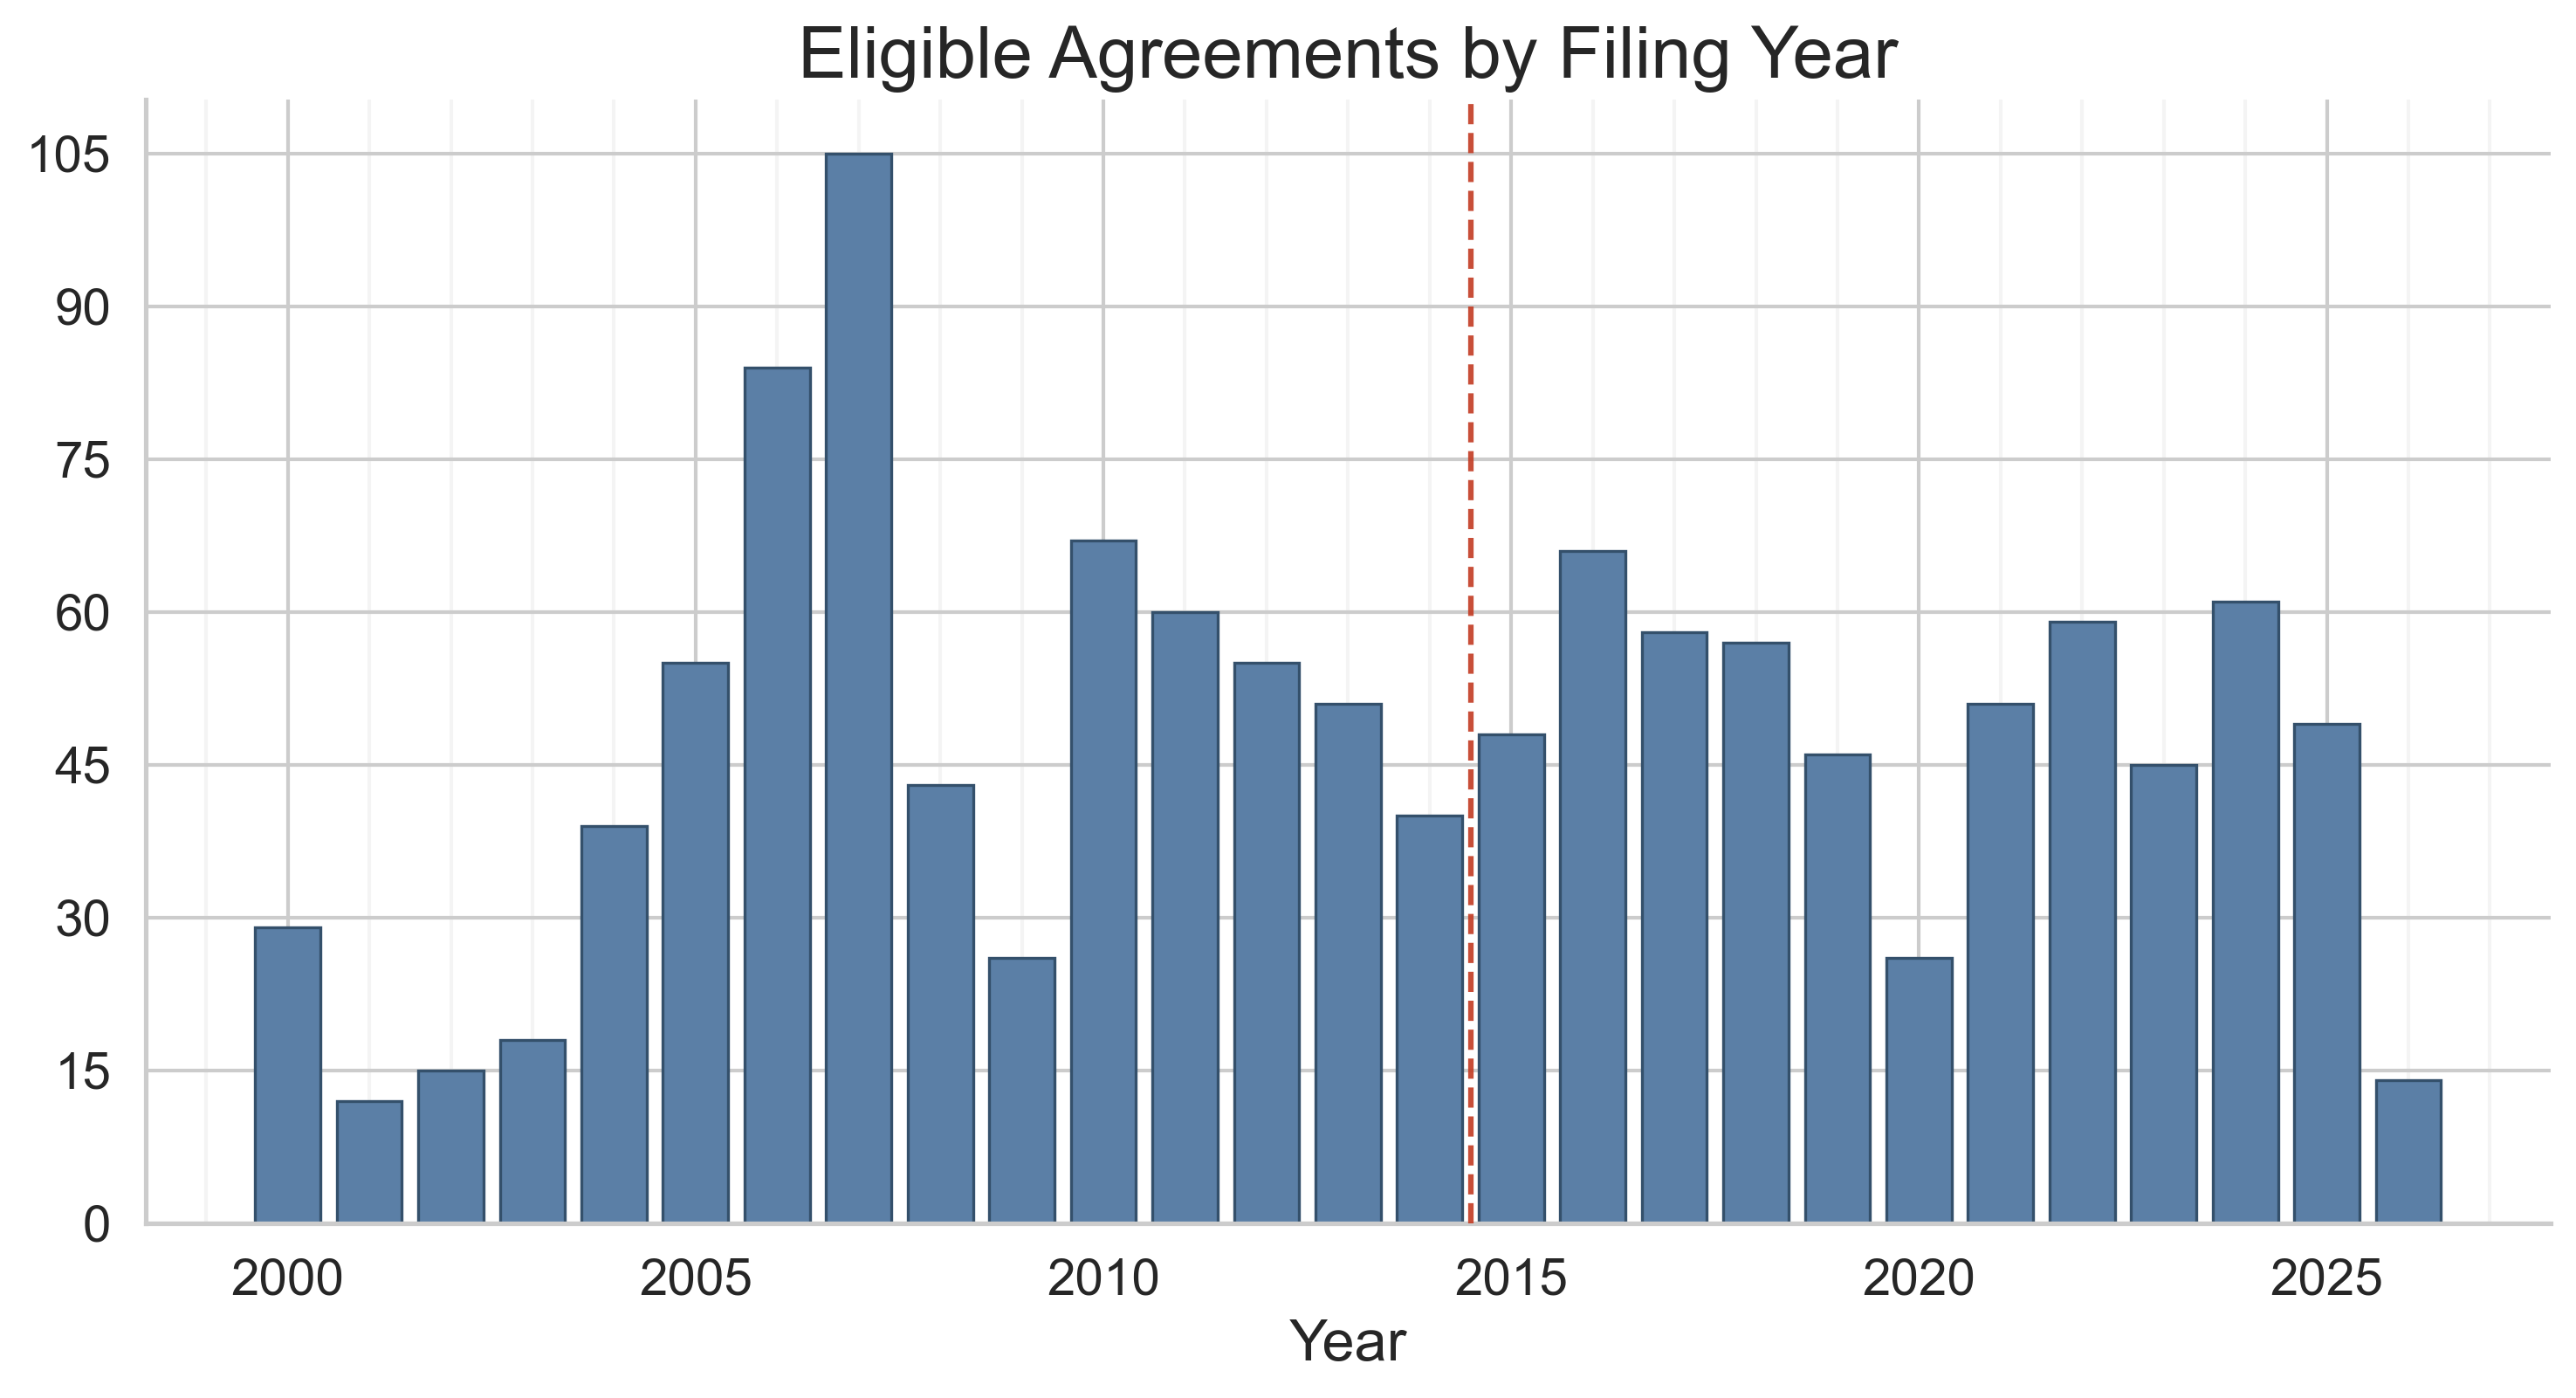
\includegraphics[width=0.92\textwidth,height=0.32\textheight,keepaspectratio]{plots/filtered_sample_agreements_by_year.png}
\caption{Eligible agreements by filing year in the filtered all-cash public-deal sample used for the forum-selection analysis.}
\label{fig:filtered-sample-agreements-by-year}
\end{figure}

\begin{figure}[H]
\centering
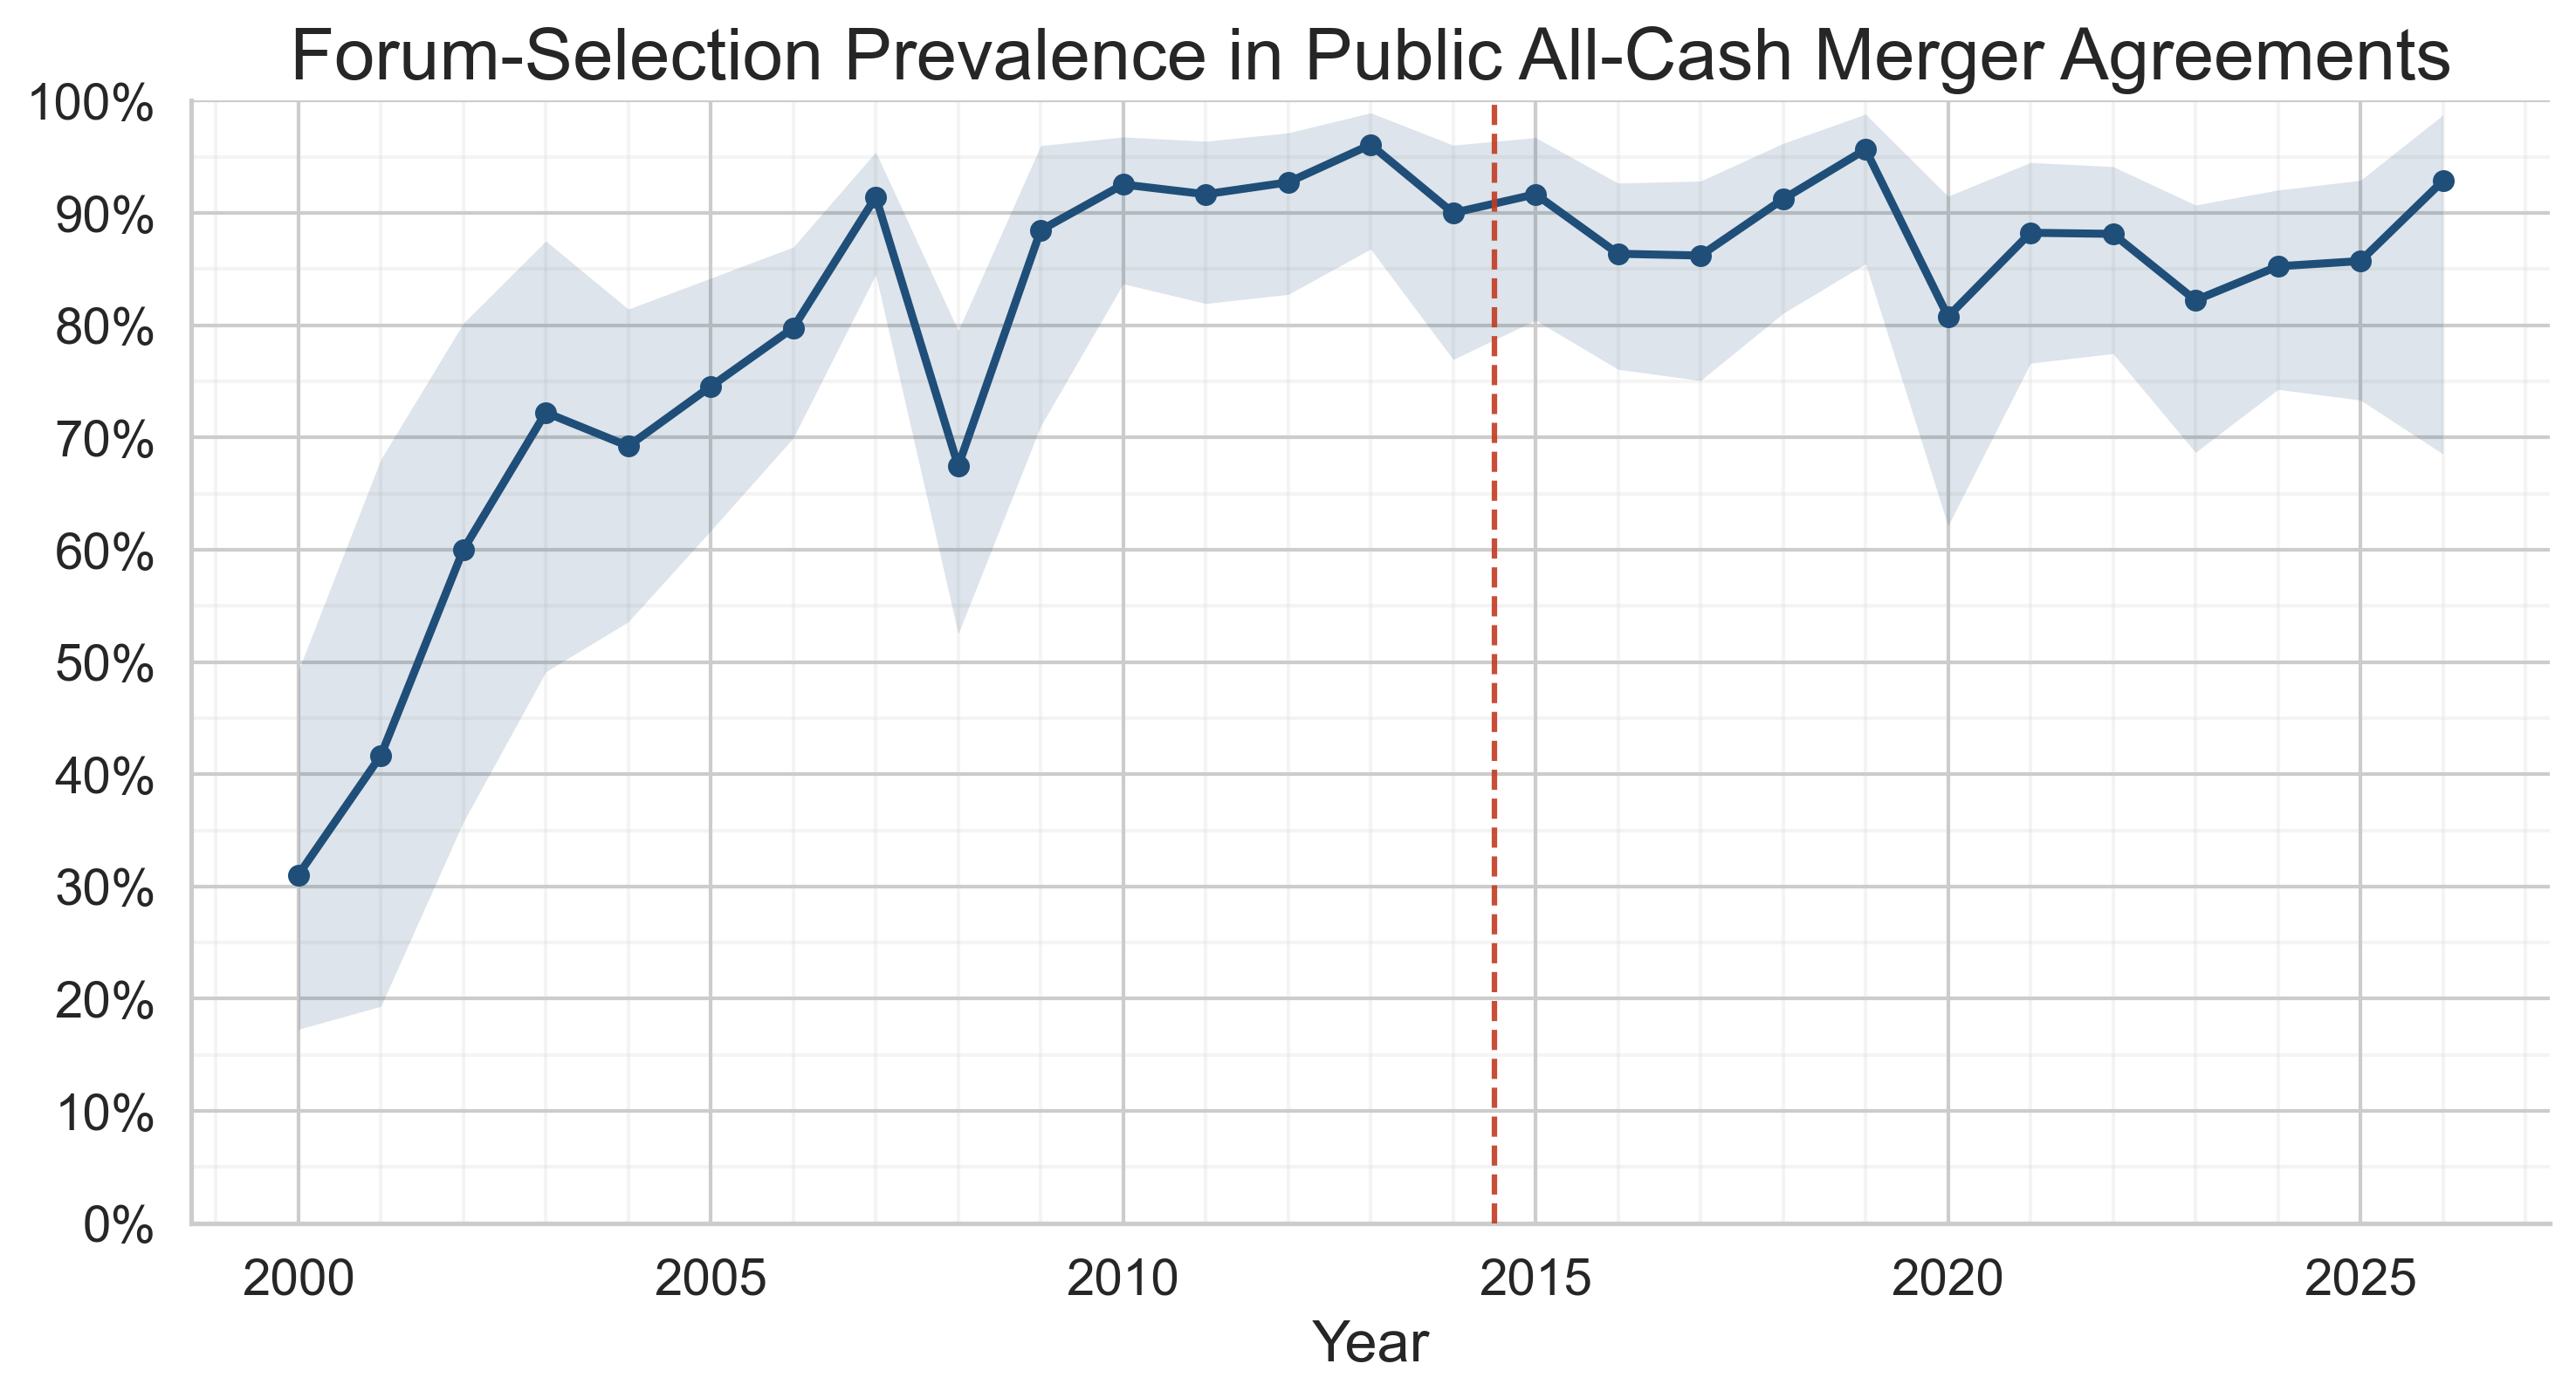
\includegraphics[width=0.92\textwidth,height=0.32\textheight,keepaspectratio]{plots/forum_clause_prevalence.png}
\caption{Forum-selection prevalence in the all-cash public-deal sample. Forum-selection clauses become common early in the sample and remain prevalent thereafter, though prevalence falls below its peak in recent years. The shaded area represents a bootstrapped 95\% confidence interval. \emph{All eligible deals + Universe A.}}
\label{fig:forum-clause-prevalence}
\end{figure}

\begin{figure}[H]
\centering
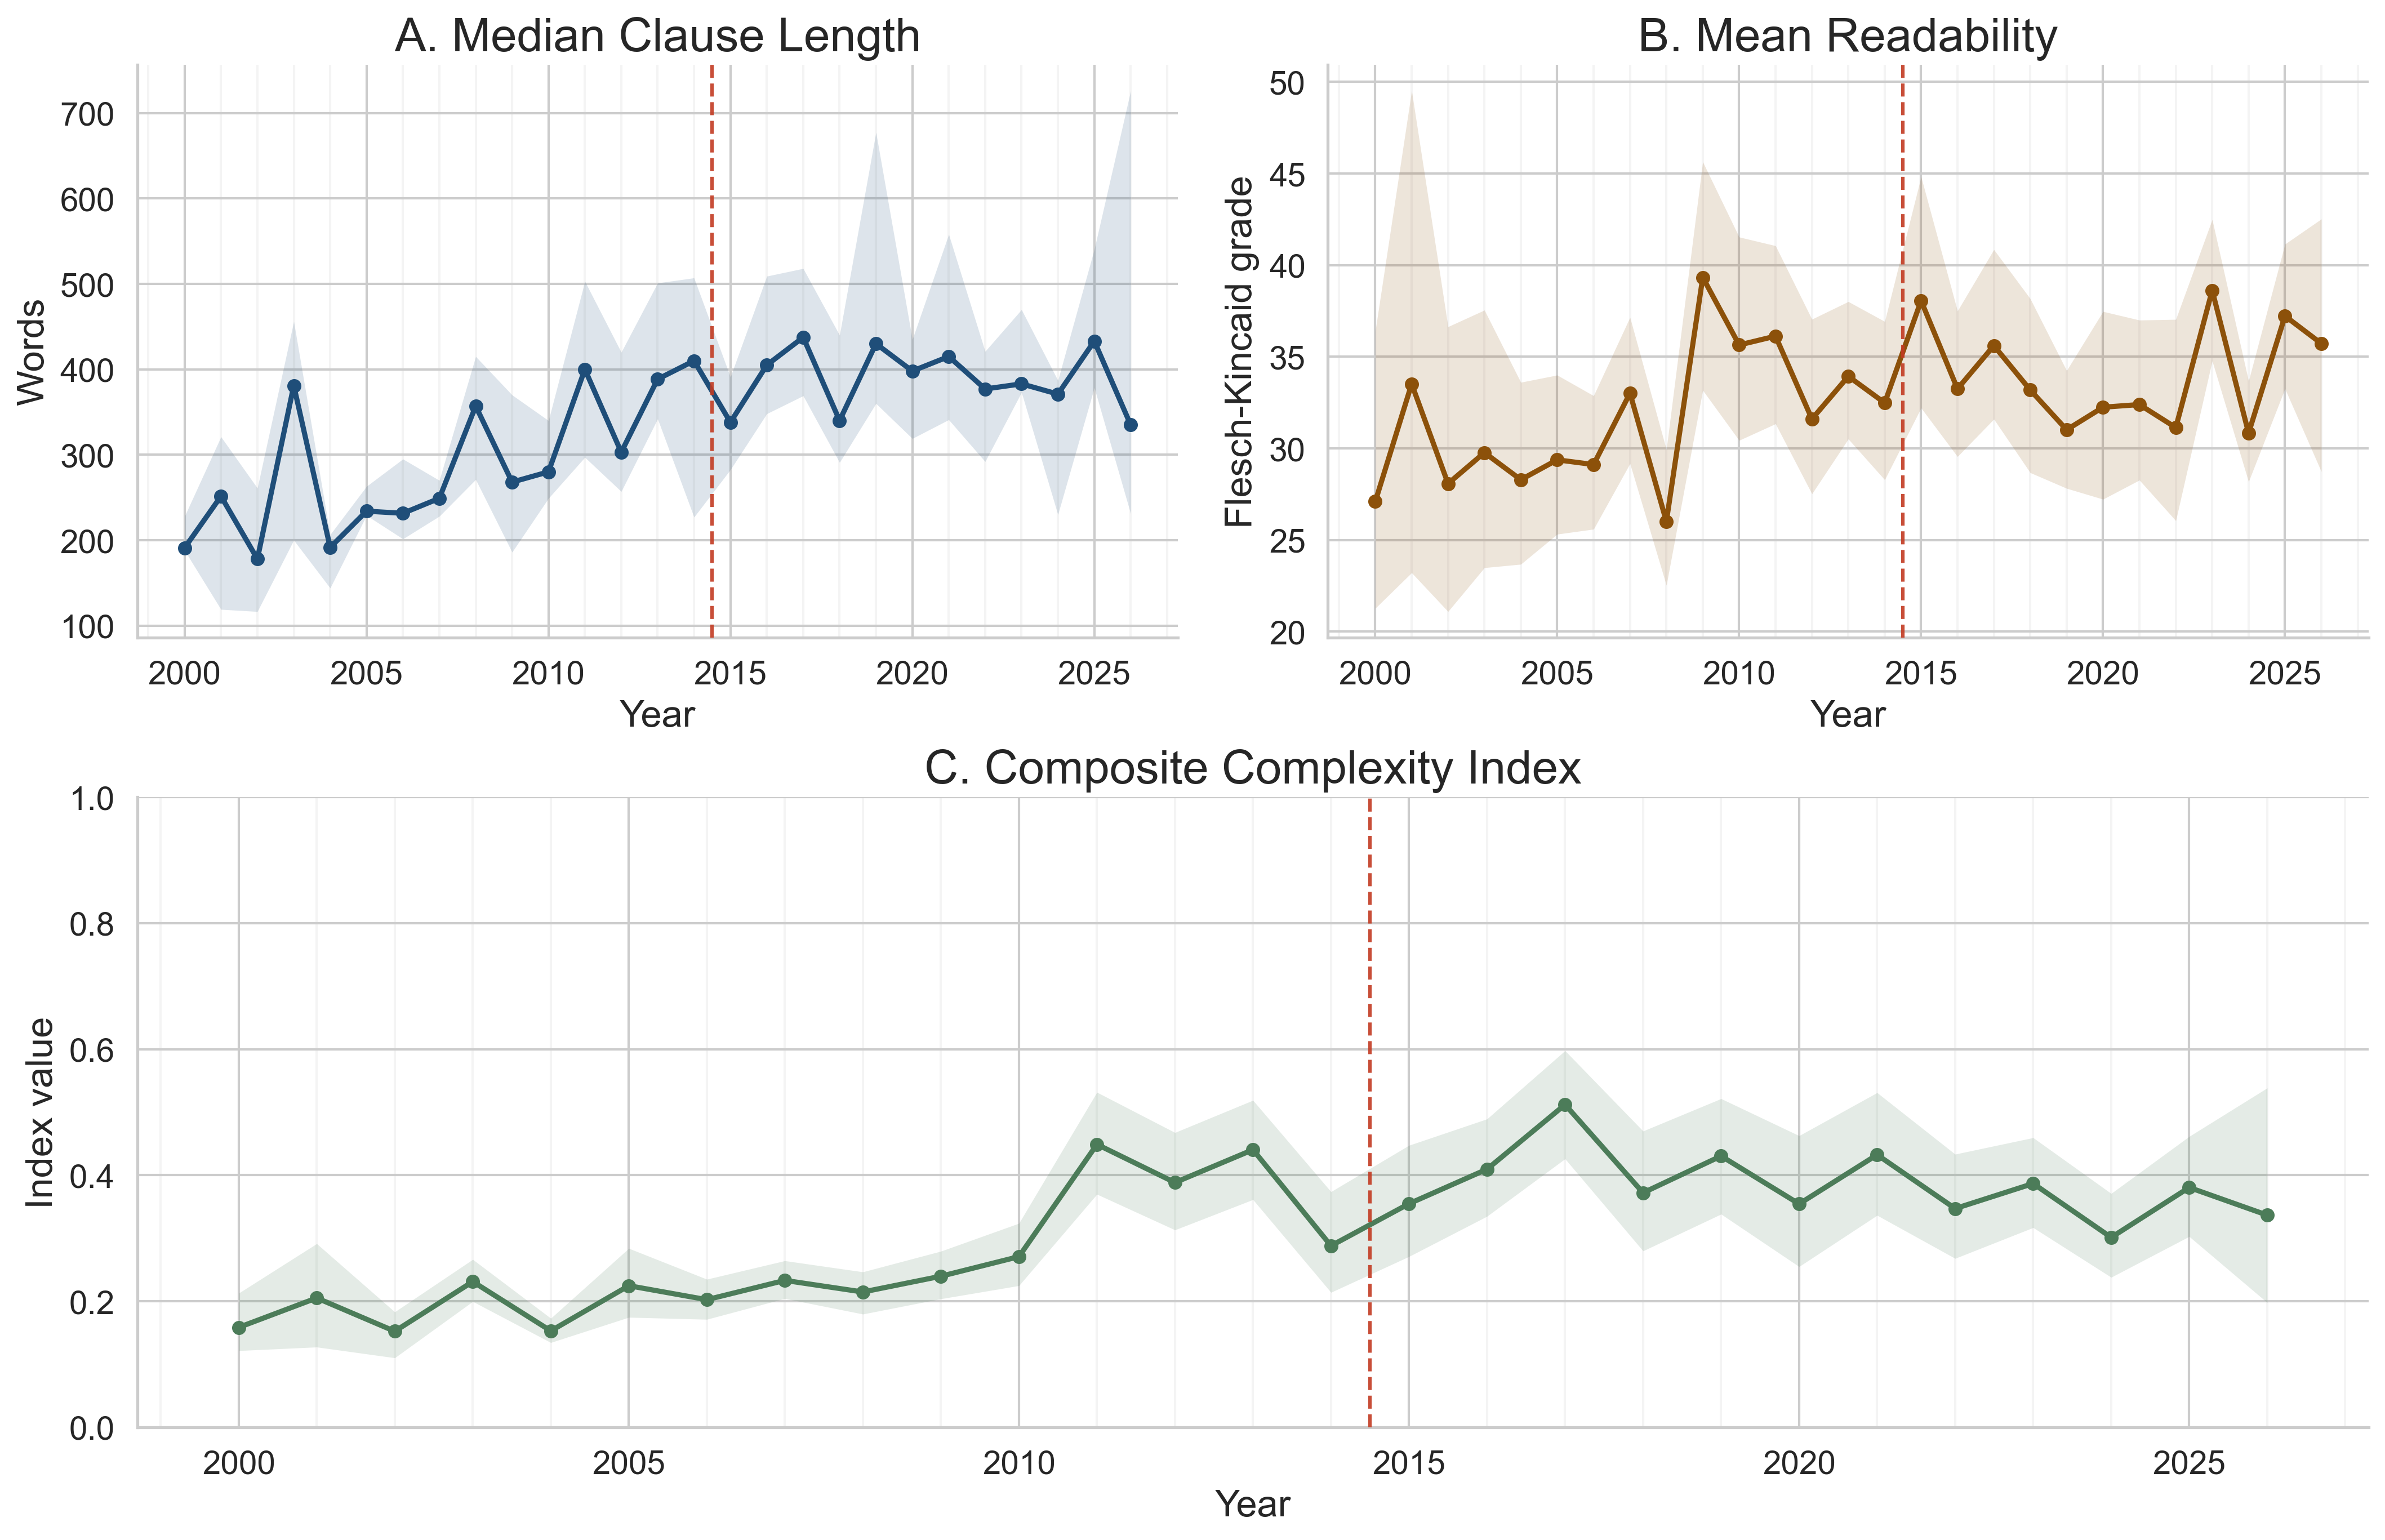
\includegraphics[width=0.92\textwidth,height=0.32\textheight,keepaspectratio]{plots/forum_clause_length_complexity.png}
\caption{Forum-selection clause length (A), readability (B), and complexity (C) over time. Each chart evidences the pattern Coates describes through 2014—increasing length and complexity. However, following 2014, median clause length, readability, and our custom proxy for complexity all plateau or even witness declines. \emph{Universe B.}}
\label{fig:forum-clause-length-complexity}
\end{figure}

\begin{figure}[H]
\centering
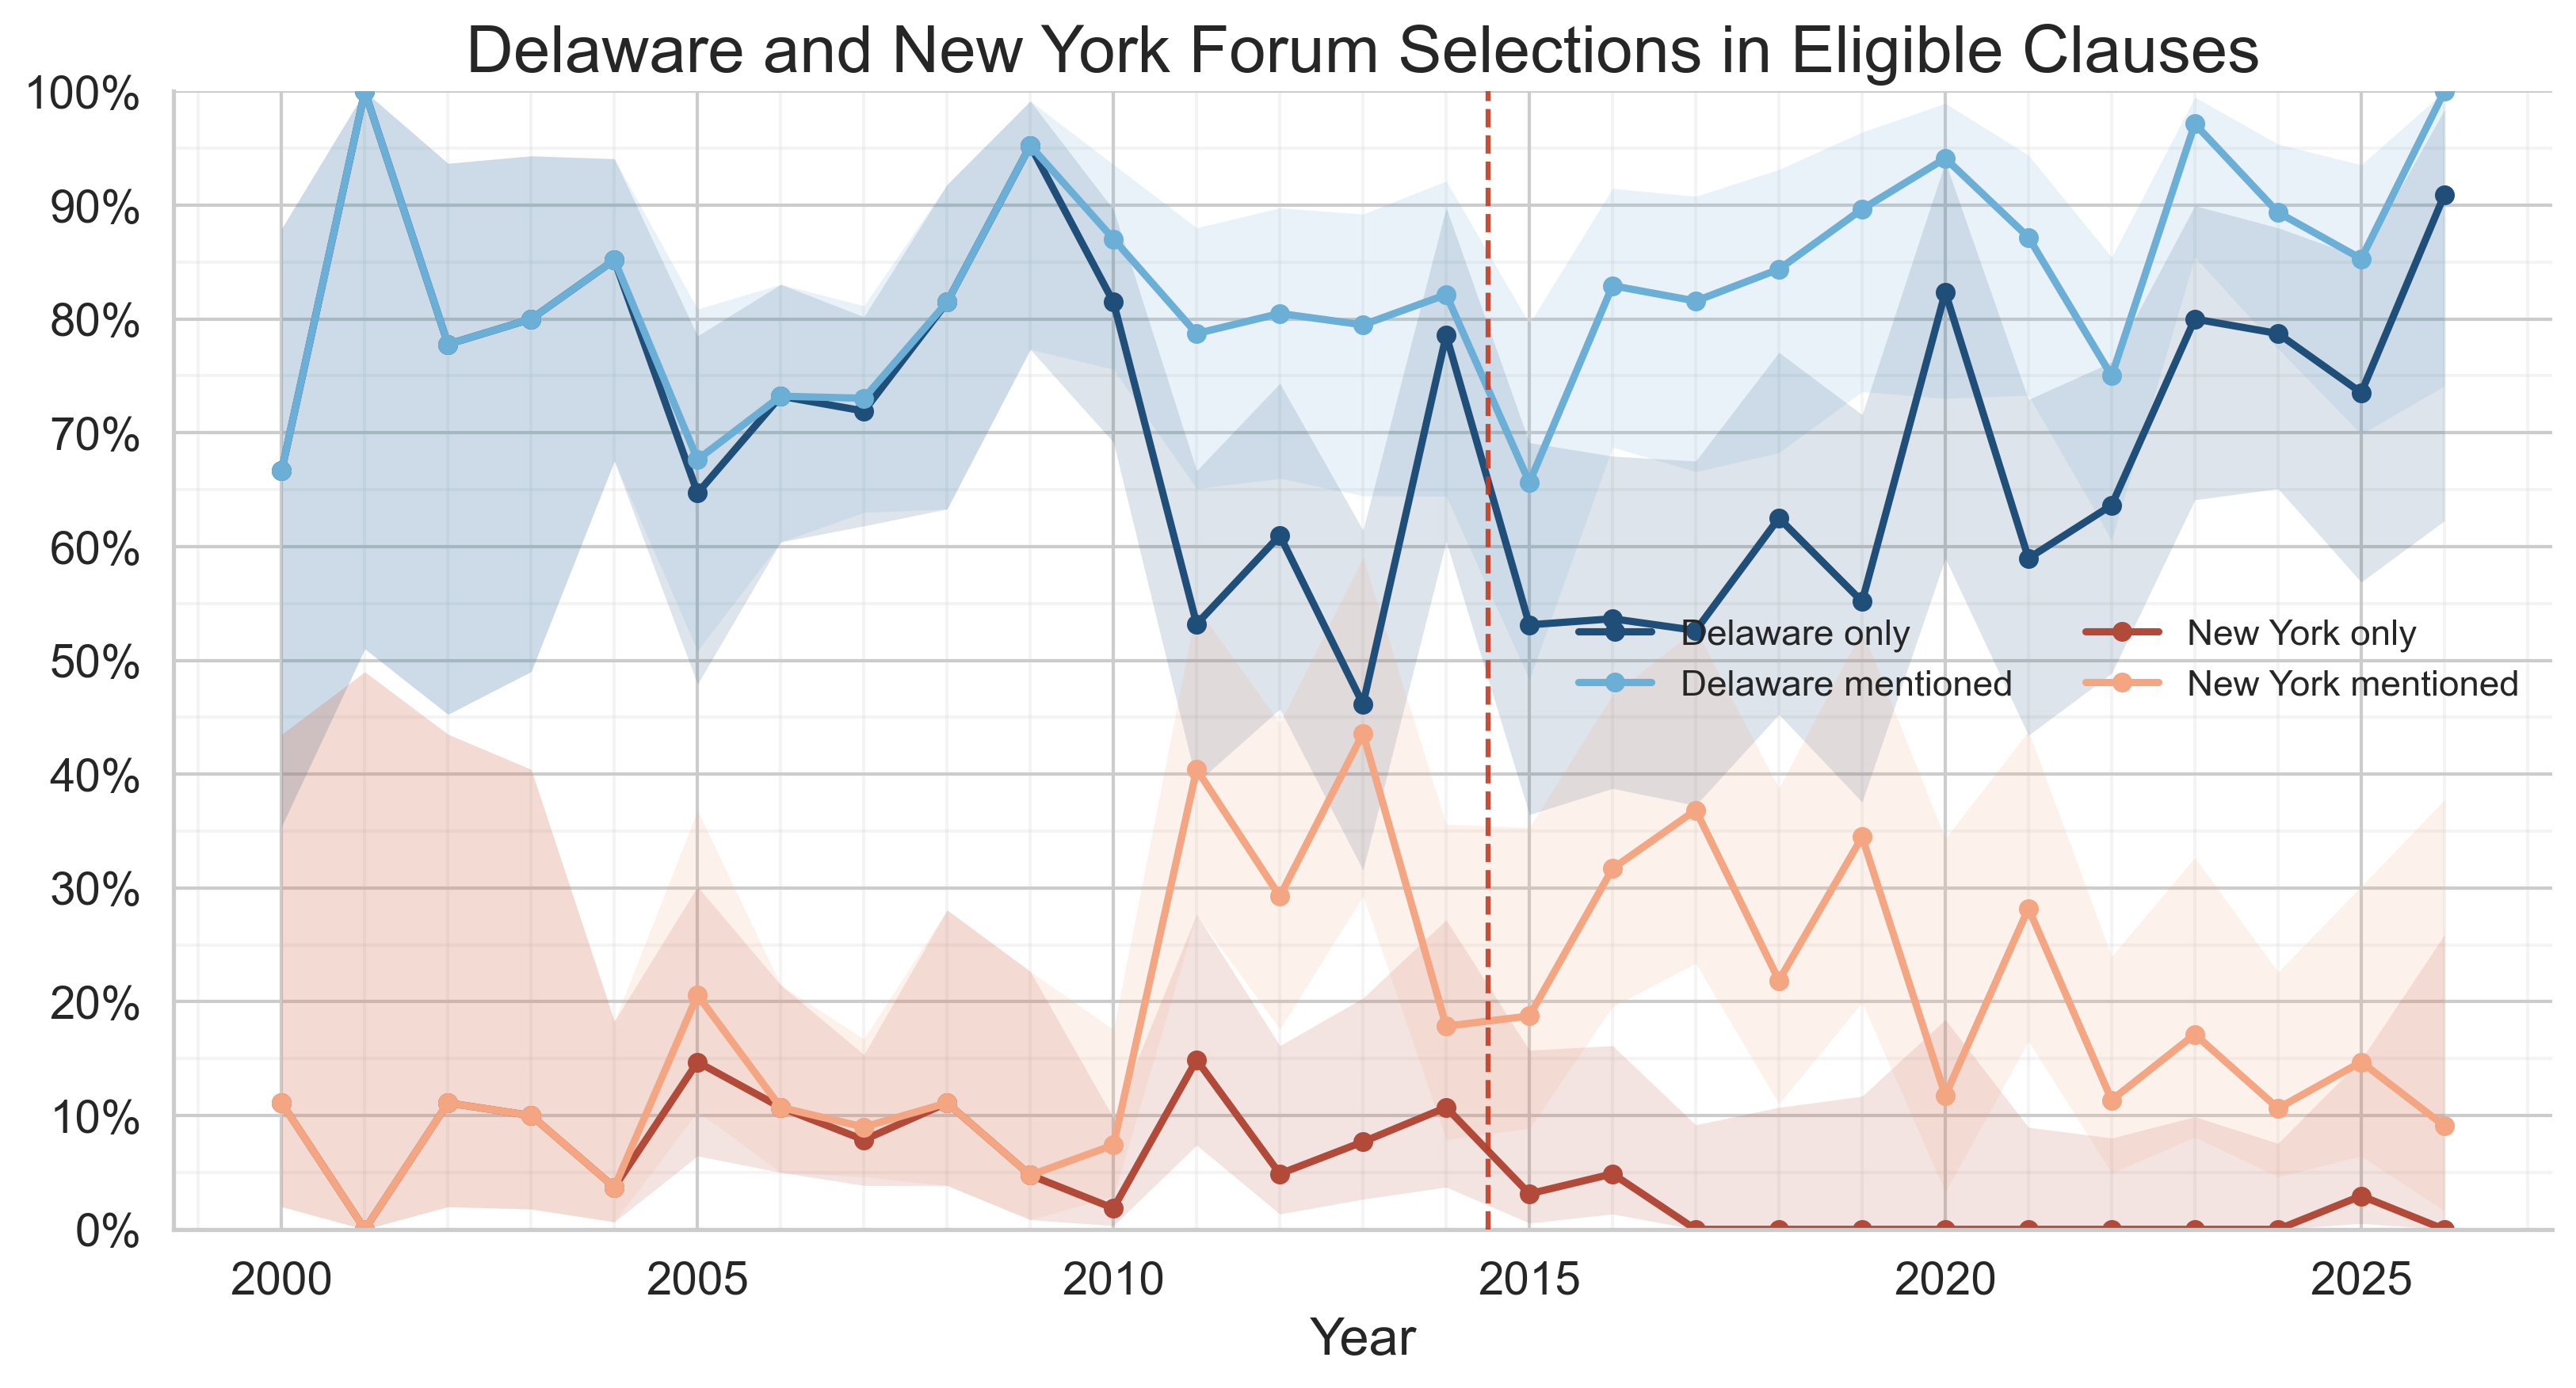
\includegraphics[width=0.92\textwidth,height=0.32\textheight,keepaspectratio]{plots/forum_clause_delaware_new_york_shares.png}
\caption{Delaware and New York shares among agreements with eligible forum-selection clauses. Delaware remains the dominant forum throughout the sample, but beginning in 2010 shares priority with New York; New York's share, however, peaks in 2013, and declines substantially in the final years of the sample. \emph{Universe A.}}
\label{fig:forum-clause-delaware-new-york}
\end{figure}

\begin{figure}[H]
\centering
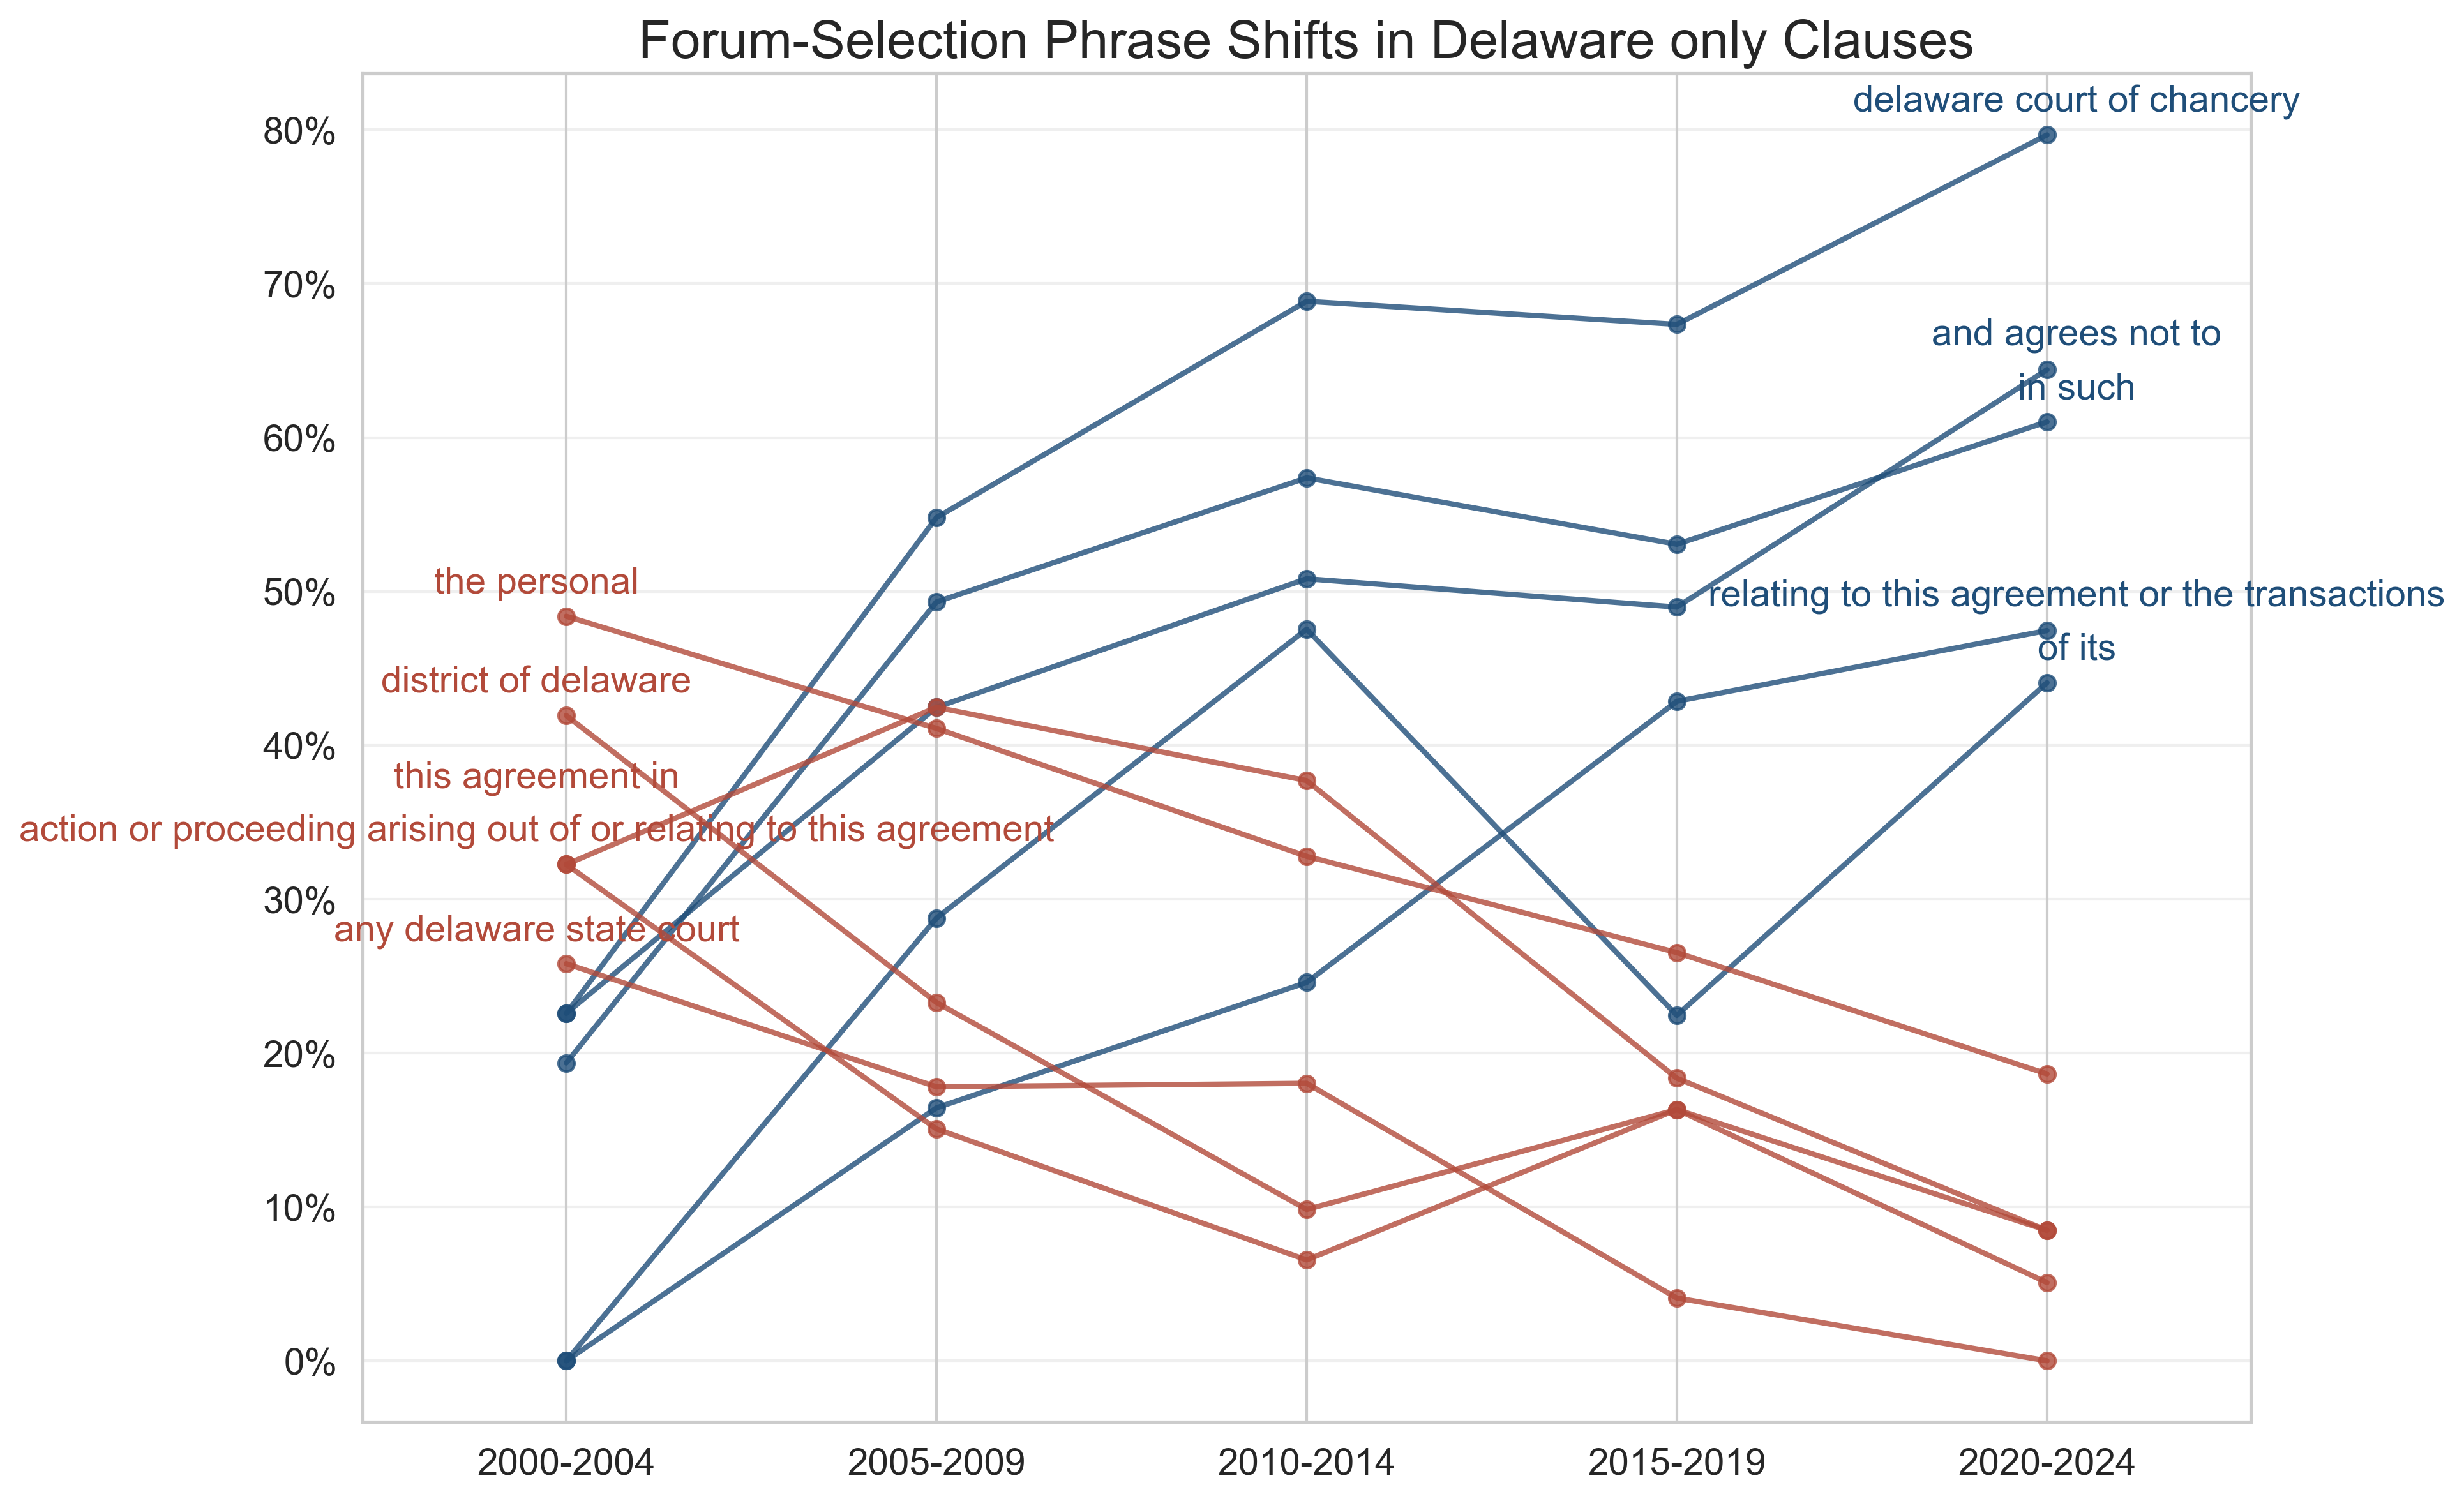
\includegraphics[width=0.92\textwidth,height=0.32\textheight,keepaspectratio]{plots/forum_clause_phrase_shift_five_periods.png}
\caption{Phrase shifts in Delaware-only forum-selection clauses across five-year periods. Note the rise of ``delaware court of chancery'' and the decline of both ``district of delaware'' and ``any delaware state court.'' Also interesting is the rise of ``relating to this agreement or the transactions,'' which did not exist at all in early-period agreements. \emph{Universe B.}}
\label{fig:forum-clause-phrase-shift-five-periods}
\end{figure}

\begin{figure}[H]
\centering
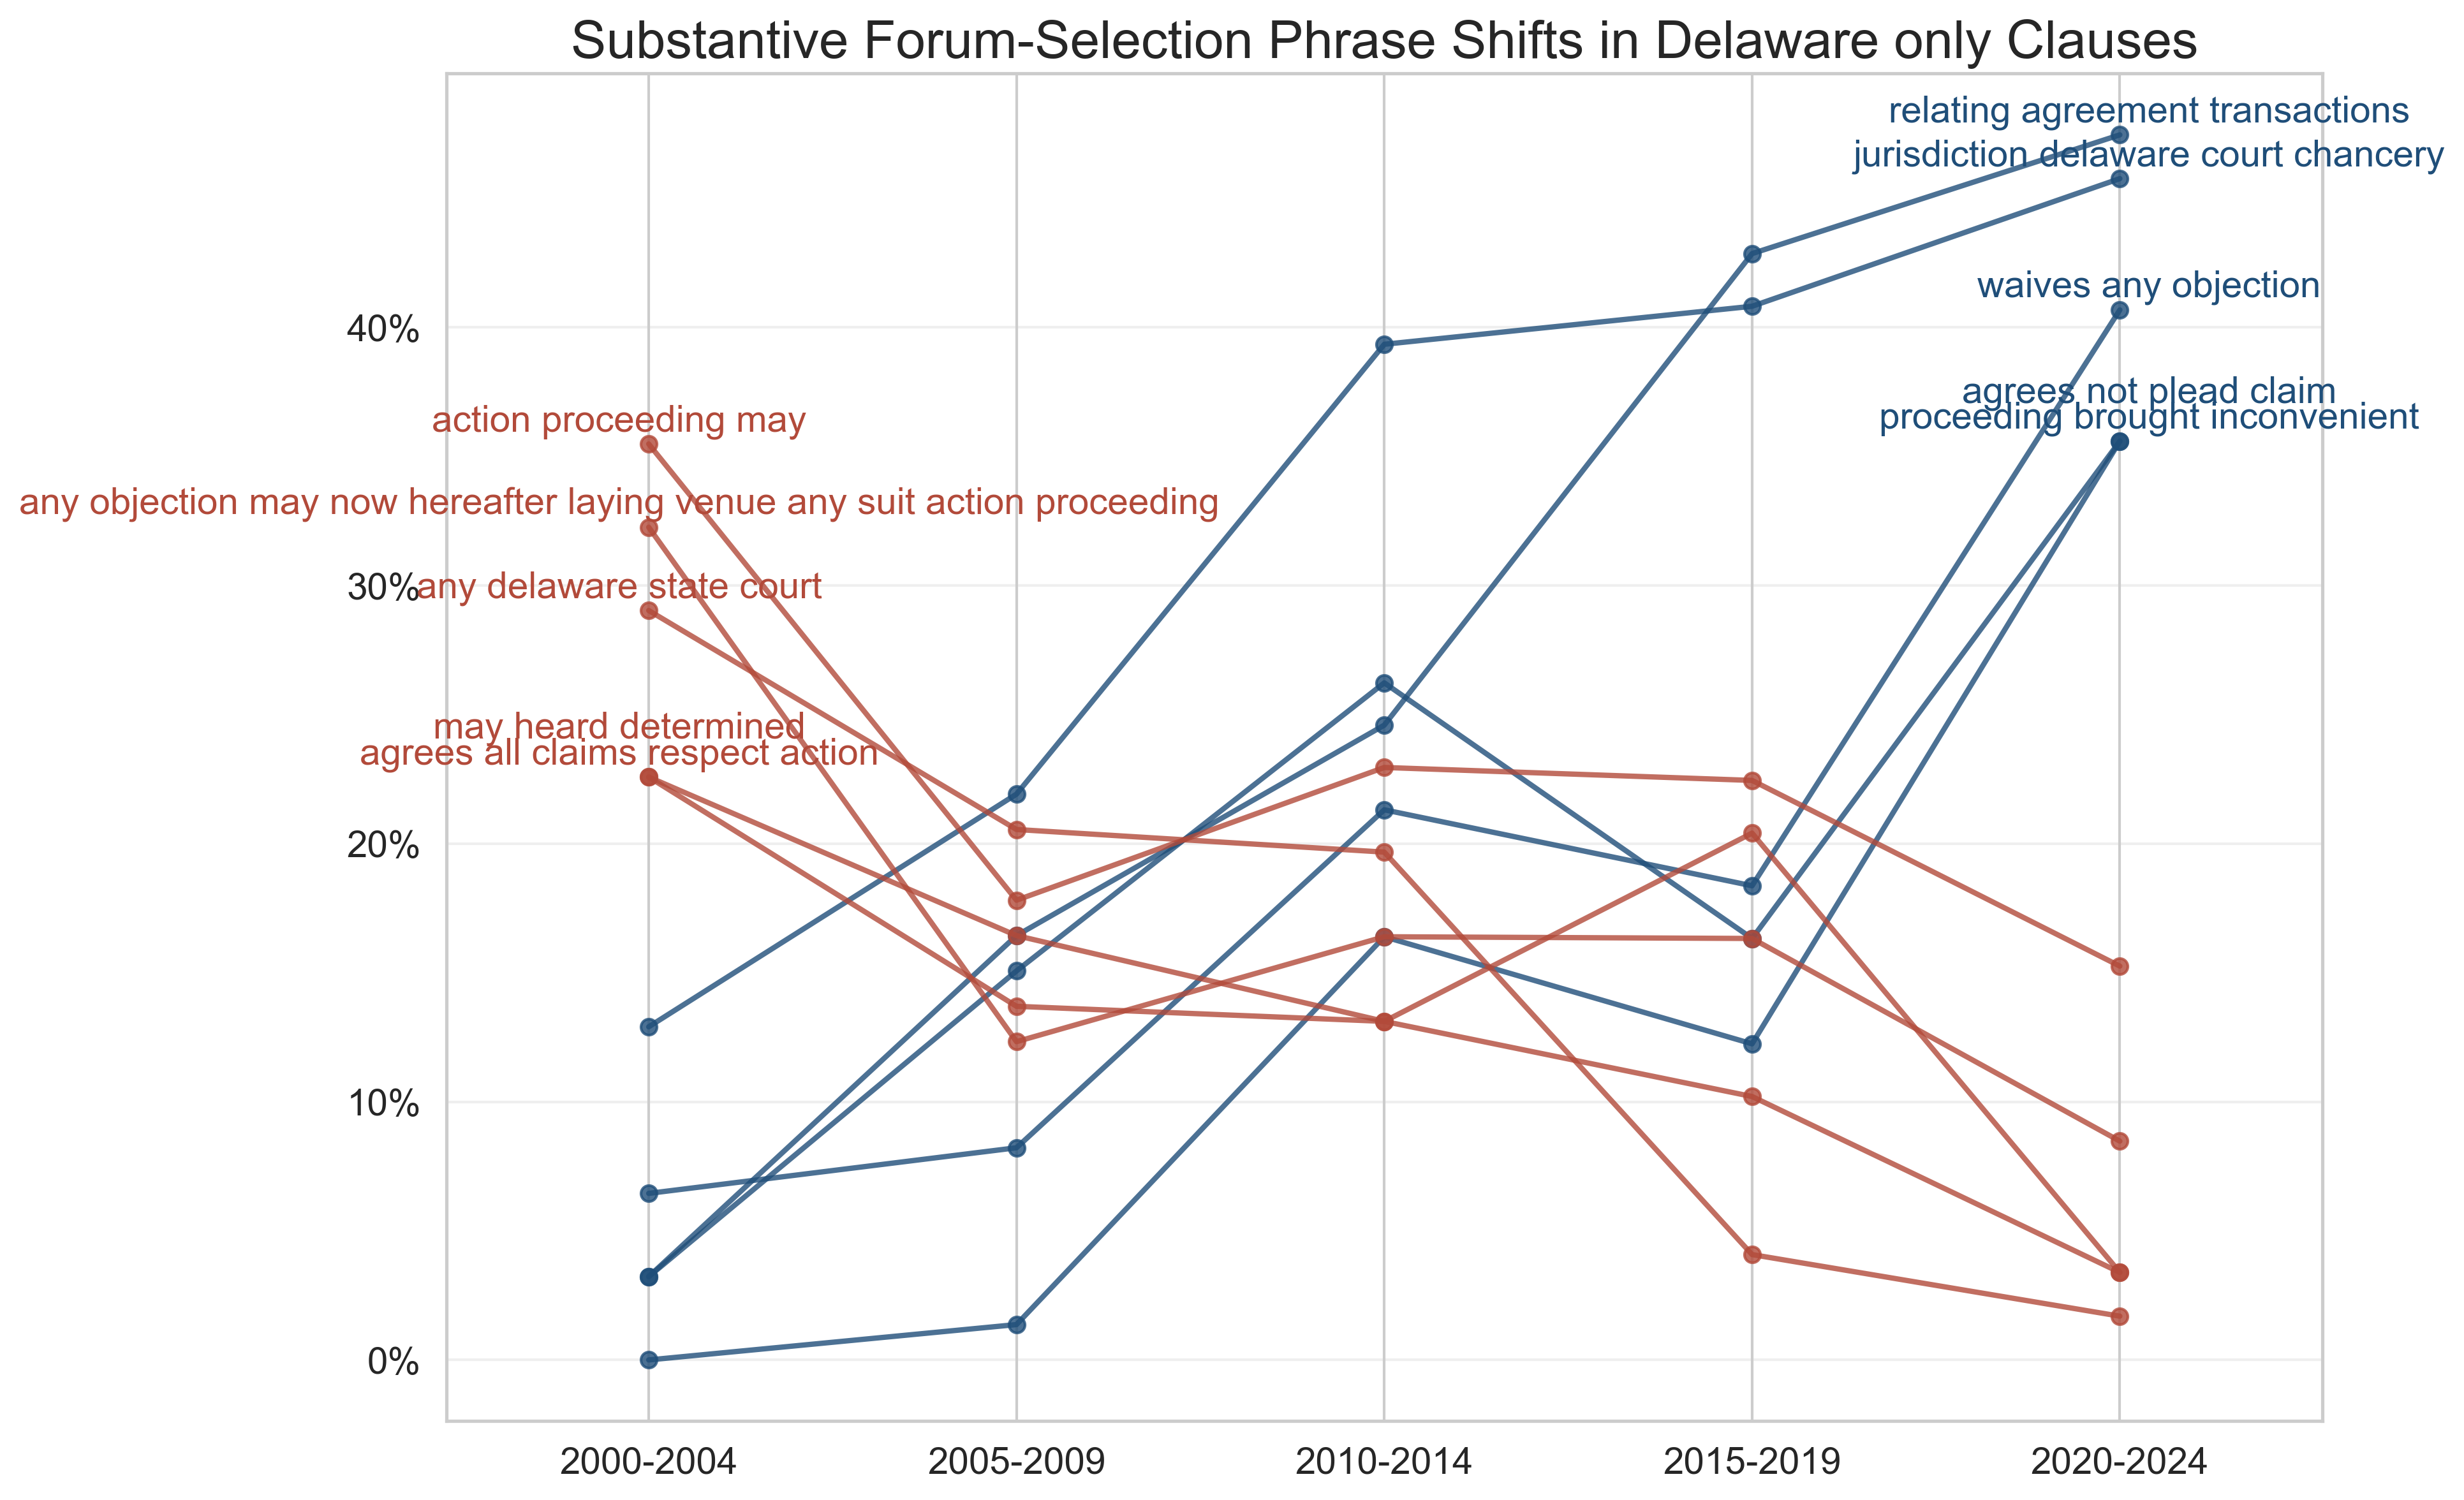
\includegraphics[width=0.92\textwidth,height=0.32\textheight,keepaspectratio]{plots/forum_clause_substantive_phrase_shift_five_periods.png}
\caption{Substantive phrase shifts in Delaware-only forum-selection clauses across five-year periods. Compared with the broader phrase plot above, this figure removes ``stop words'' to focus (ideally) on differences in substantive phrases. Similar to above, we can see here the rising preference for Chancery Court over just any Delaware court, and the rise of ``related transactions'' language. \emph{Universe B.}}
\label{fig:forum-clause-substantive-phrase-shift-five-periods}
\end{figure}

\section{Conclusion}
In this paper, we introduce Pandects, the first open-source database of structured M\&A agreements. Building on the DMA Corpus, we make public over 9,000 M\&A agreements filed on EDGAR between January 1, 2000 and April 10, 2026—with monthly updates hereafter. Our pipelines, which like the rest of this project are open-source, transform agreements into structured XML, taxonomize their sections into a comprehensive taxonomy, and enrich them with deal metadata, after which we make the data available in an online UI, via API, as a bulk download of the source database, and via MCP server. Simultaneously, we make available a directory of example Jupyter Notebooks and a comprehensive documentation site for the API. Finally, we use Pandects data and APIs to confirm and update John Coates' study of forum selection clauses, demonstrating one way in which quantitative researchers can utilize Pandects data.

\newpage
\begin{appendices}
\section{Transaction Metadata Fields}\label{app:transaction-metadata}

\begingroup
\singlespacing
\begin{center}
\small
\begin{longtable}{p{0.22\textwidth}p{0.42\textwidth}p{0.28\textwidth}}
\caption{Agreement-level transaction metadata fields.} \\
\toprule
Field & Description & Validation \\
\midrule
\endfirsthead

\toprule
Field & Description & Validation \\
\midrule
\endhead

\bottomrule
\endfoot

Transaction Price Total & Total transaction value when available. & Derived from component values. For mixed consideration, total is populated only when at least two non-null components are present. \\
Transaction Price Cash & Cash portion of transaction consideration. & Numeric, non-negative, or null. Must be null when price is stated only in non-USD terms. \\
Transaction Price Stock & Stock portion of transaction consideration. & Numeric, non-negative, or null. Must be null when price is stated only in non-USD terms. \\
Transaction Price Assets & Asset or other non-cash, non-stock portion of transaction consideration. & Numeric, non-negative, or null. Must be null when price is stated only in non-USD terms. \\
Transaction Consideration & High-level consideration classification. & One of cash, stock, or mixed in the database; null when unknown. Must be consistent with the non-zero price components. \\
Target Type & Whether the target was public or private at announcement. & One of public or private, or null if unresolved. \\
Acquirer Type & Whether the acquirer was public or private at announcement. & One of public or private, or null if unresolved. \\
Target Private Equity & Whether the target was private-equity backed. & Boolean or null. \\
Acquirer Private Equity & Whether the acquirer was a private-equity buyer. & Boolean or null. \\
Target Industry & Target industry classification. & Two- or three-digit NAICS code, or null. \\
Acquirer Industry & Acquirer industry classification. & Two- or three-digit NAICS code, or null. \\
Announcement Date & Public announcement date for the transaction. & Valid YYYY-MM-DD date, or null. \\
Close Date & Transaction closing date, when available. & Valid YYYY-MM-DD date, or null; cannot precede Announcement Date. \\
Deal Status & Current status of the transaction. & One of pending, complete, or cancelled, or null if unresolved. Complete requires a non-null Close Date; pending requires Close Date to be null. \\
Attitude & High-level deal attitude classification. & One of friendly, hostile, or unsolicited, or null. \\
Deal Type & High-level transaction form. & One of merger, stock acquisition, asset acquisition, tender offer, or membership interest purchase, or null. \\
Purpose & High-level buyer motivation. & One of strategic or financial, or null. \\
\end{longtable}
\end{center}
\endgroup
\normalsize

\section{Forum Selection Excerpts}
\label{app:clause-excerpts}
\subsection{Selecting both Delaware and New York}
\label{app:excerpt-de-ny}
\begingroup
\singlespacing
\begin{quote}
  Each of the parties hereto hereby expressly, irrevocably and unconditionally submits, for itself and its property, to the exclusive jurisdiction of the Court of Chancery of the \strong{State of Delaware} or, if such court shall not have jurisdiction, any Federal court of the United States of America sitting in \strong{Delaware}, and any appellate court from any appeal thereof, in any Proceeding arising out of or relating to this Agreement or the agreements delivered in connection herewith or the Transactions contemplated hereby or thereby or for recognition or enforcement of any judgment relating thereto, and each of the parties hereby irrevocably and unconditionally.... Notwithstanding anything herein to the contrary, each of the parties hereto agrees (i) that any Proceeding of any kind or nature, whether at law or in equity, in contract, tort or otherwise, against a Financing Source in connection with this Agreement, the Debt Financing, the Preferred Equity Financing or the Transactions, shall be subject to the exclusive jurisdiction of any state or federal court sitting in the Borough of Manhattan, \strong{New York, New York} and any appellate court thereof and each party hereto submits for itself and its property with respect to any such Proceeding to the exclusive jurisdiction of such courts...\footnote{Excerpted from the agreement for the 2018 acquisition of Cotiviti Holdings, Inc. by Veritas Capital Fund Management LLC; Verscend Technologies, Inc. Pandects agreement UUID 9670100e-e34c-59c4-a85a-aca44ea7edb9.}
\end{quote}
\endgroup

\subsection{Selecting the Chancery Court}
\label{app:excerpt-chancery}
An example early-period forum selection clause, which selects ``any Delaware state court.''
\begingroup
\singlespacing
\begin{quote}
  Any suit, action or proceeding seeking to enforce any provision of, or based on any matter arising out of or in connection with, this Agreement or the transactions contemplated hereby may be brought in any federal court located in the State of Delaware or \strong{any Delaware state court}, and each of the parties hereby consents to the jurisdiction of such courts (and of the appropriate appellate courts therefrom) in any such suit, action or proceeding and irrevocably waives, to the fullest extent permitted by Law....\footnote{Excerpted from the agreement for the 2000 acquisition of Keebler Foods Co. by Kellogg Co. Pandects agreement UUID 9a43c28f-bade-5c4d-9953-431e10ab7053.}
\end{quote}
\endgroup

An example late-period forum selection clause, which expressly privileges ``the Court of Chancery of the State of Delaware.''
\begingroup
\singlespacing
\begin{quote}
  Each of the parties hereto ... (b) irrevocably and unconditionally consents and submits itself and its properties and assets in any action or proceeding to the exclusive jurisdiction of the \strong{Court of Chancery of the State of Delaware} (or, only if the Court of Chancery of the State of Delaware declines to accept or does not have jurisdiction over a particular matter, any federal or other state court sitting in New Castle County within the State of Delaware) in the event any dispute or controversy arises out of this Agreement or the transactions contemplated hereby, or for recognition and enforcement of any judgment in respect thereof; ... (d) agrees that any actions or proceedings arising in connection with this Agreement or the transactions contemplated hereby shall be brought, tried and determined only in the \strong{Court of Chancery of the State of Delaware} (or, only if the Court of Chancery of the State of Delaware declines to accept or does not have jurisdiction over a particular matter, any federal or other state court sitting in New Castle County within the State of Delaware)....\footnote{Excerpted from the agreement for the 2020 acquisition of Biospecifics Technologies Corp. by Endo International Plc. Pandects agreement UUID 0ccdac8a-f969-5e68-aaab-8f42829710a6.}
\end{quote}
\endgroup

\subsection{Covering Related Transactions}
\label{app:excerpt-related-tx}
An example early-period forum selection clause, which contemplates disputes arising out of the given agreement only.
\begingroup
\singlespacing
\begin{quote}
  Each of the parties to this Agreement submits to the jurisdiction of any state or federal court sitting in the State of Delaware, in any action or proceeding \strong{arising out of or relating to this Agreement}, agrees that all claims in respect of the action or proceeding may be heard and determined in any such court, and agrees not to bring any action or proceeding \strong{arising out of or relating to this Agreement} in any other court. Each of the parties to this Agreement waives any defense of inconvenient forum to the maintenance of any action or proceeding so brought and waives any bond, surety or other security that might be required of any other party with respect thereto.\footnote{Excerpted from the agreement for the 2001 acquisition of Newport News Shipbuilding, Inc. by General Dynamics Corp. Pandects agreement UUID 72dc0cdb-c625-59de-aeeb-d1a860574b13.}
\end{quote}
\endgroup

An example late-period forum selection clause, which uses the expanded ``transactions contemplated hereby'' locution.
\begingroup
\singlespacing
\begin{quote}
  Each of the parties irrevocably agrees that any legal action or proceeding \strong{arising out of or relating to this Agreement} brought by any party or its Affiliates against any other party or its Affiliates shall be brought and determined in the Court of Chancery of the State of Delaware... Each of the parties hereby irrevocably submits to the jurisdiction of the aforesaid courts for itself and with respect to its property, generally and unconditionally, with regard to any such action or proceeding \strong{arising out of or relating to this Agreement and \underline{\smash{the transactions contemplated hereby}}}, including the Merger.... Each of the parties hereby irrevocably and unconditionally waives, and agrees not to assert, by way of motion or as a defense, counterclaim or otherwise, in any action or proceeding \strong{arising out of or relating to this Agreement or \underline{\smash{the transactions contemplated hereby}}}, including the Merger....\footnote{Excerpted from the agreement for the 2020 acquisition of Foundation Building Materials, Inc. by American Securities LLC. Pandects agreement UUID 33afdf7b-be11-5b18-bf61-1e12193a0fa5.}
\end{quote}
\endgroup

\section{LLM Prompts}
\label{app:llm-prompts}

This appendix reproduces the operative LLM ``system'' prompts in use as of 4/28/2026. The prompt in \autoref{app:training-data-prompt} is static, since it was used solely for generating NER training data; all other prompts are subject to change, and the latest versions will always be in the GitHub repository.

\subsection{Article and Section Tagging}

\subsubsection{NER Training-Data Prompt}
\label{app:training-data-prompt}
\begingroup
\singlespacing
\begin{minted}[breaklines,breakanywhere,fontsize=\scriptsize]{text}
# Identity

You are a professional data tagger. You will be reviewing and tagging individual pages from Merger & Acquisition agreements.

# Instructions

Your task is to place a <section></section> tag around section HEADINGS (the number and title) and an <article></article> tag around article HEADINGS (the number and title). The tags should encompass the number AND heading title, but NOT the body text of the section or article itself. REFERENCES to sections and article--rather than headings--should never be tagged. Once again, your task is to tag HEADINGS; you will ignore REFERENCES. Be attentive to context to ensure accuracy. 

Finally, many pages have a number at either the very beginning or the very end; this number corresponds to the page of the agreement. If you see a number at the very begining [sic] or end of a page and that number, in context, looks like it could be a page number, enclose that number in a <page></page> tag. Very ocassionally [sic] you'll see two numbers at the start or end; in those cases, the "inner most" number—second number, on top; first number, on bottom—is the "real" page number. Page numbers are always integers between 1 and 300, but may have a hyphen before/after them, which you can include in the tag.

Return only the original text plus the tags, if any. Do not make any modifications outside of adding tags. Do not change punctuation, capitalization, whitespace, line breaks, or wording. Do not normalize text. Do not insert newlines. Do not correct formatting.

Some additional notes:
* Articles and sections will never occur mid-sentence. REFERENCES to articles and sections, however, typically will be mid-sentence.
* Articles will almost always be preceeded [sic] by the word "Article" and may look like "Article I   Representations" or "Article 1  Warranties"
* Sections will often but not always be preceeded [sic] by the word "Section"; sometimes they will be just numbers, like "5.01   Company Representations", and sometimes they will just be numbers (which should be tagged) followed by the section body (which should not be tagged), like "5.01"
* If you are placing an <article> or <section> tag around long sentences, you're probably doing something wrong, like confusing the section body for the heading title.
* Sub-sections do NOT count as sections and should NOT be tagged. E.g., "9.2.1" is NOT a section; instead, you would tage [sic] "9.2" (and any associated heading), which would appear somewhere above 9.2.1., but possibly not on the page you have. If only a subsection appears on the page and the parent section heading is NOT present, do not invent or infer it. Simply do not tag, consistent with the principle that sub-sections don't get tags.
* Sometimes there will be lots of extra spaces between the word "Section" or "Article" and the heading's title. This is fine and should not affect your decision to tag or not tag.
* Sometimes you will encounter long sections of definitions, where terms in double quotes are juxtaposed to section or article references, such as in: “Disposition Actions”\n\nSection 8(d)\n\n. Context should help you avoid mistakenly tagging article or section references in these definitions pages. A crude rule of thumb is that, if you are tagging an article or section and the text before and after it is in double quotes, you're probably doing something wrong.

# Examples

<page_snippet>
... any Ancillary Agreement or the transactions contemplated hereby or thereby. 10.19 Mutual Drafting. This Agreement and the Ancillary Agreements shall be deemed...
<page_snippet>

<assistant_response>
... any Ancillary Agreement or the transactions contemplated hereby or thereby. <section>10.19 Mutual Drafting.</section> This Agreement and the Ancillary Agreements shall be deemed...
</assistant_response>

<page_snippet>
... Acceptance Time and all filings and notifications described in Section 5.4(b) will have been made and any waiting periods thereunder will have terminated or expired...
</page_snippet>

<assistant_response>
... Acceptance Time and all filings and notifications described in Section 5.4(b) will have been made and any waiting periods thereunder will have terminated or expired...
</assistant_response>

<page_snippet>
NOW, THEREFORE, the parties hereto agree as follows:    ARTICLE 1    DEFINITIONS    Section 1.01. Definitions. (a) As used herein, the following terms have the following meanings:    “ 1934 Act ” means the Securities Exchange Act of 1934.
</page_snippet>

<assistant_response>
NOW, THEREFORE, the parties hereto agree as follows:    <article>ARTICLE 1    DEFINITIONS</article>    <section>Section 1.01. Definitions.</section> (a) As used herein, the following terms have the following meanings:    “ 1934 Act ” means the Securities Exchange Act of 1934.
</assistant_response>

<page_snippet>
... 19.9 Representations of the Company 19.7.1 The Company hereby warrants and represents that it shall not modify its operations outside of the ordinary course of business during the time...
</page_snippet>

<assistant_response>
... <section>19.9 Representations of the Company</section> 19.7.1 The Company hereby warrants and represents that it shall not modify its operations outside of the ordinary course of business during the time...
</assistant_response>

<page_snippet>
... 10.1 The purchase price for the Purchased Assets and the Shares is (i) One Hundred and Twenty Million U.S. Dollars ($120,000,000),  plus  or  minus , as applicable...
</page_snippet>

<assistant_response>
... <section>10.1</section> The purchase price for the Purchased Assets and the Shares is (i) One Hundred and Twenty Million U.S. Dollars ($120,000,000),  plus  or  minus , as applicable...
</assistant_response>
\end{minted}
\endgroup

\subsubsection{Full-Page AI Repair Prompt}
\label{app:ai-repair-prompt}
\begingroup
\singlespacing
\begin{minted}[breaklines,breakanywhere,fontsize=\scriptsize]{text}
# Identity

You are a professional data tagger. You will be reviewing and tagging individual pages from Merger & Acquisition agreements.

# Instructions

First things first, if the page appears to be: 1) front matter; 2) part of the Table of Contents; 3) part of any signatures block sections; 4) part of a disclosure schedule in the Exhibits section; or 5) otherwise not from the main agreement, do not add tags. This will be the case rarely, if at all. Note that the recitals section IS part of the main agreement and should NOT be skipped; the recitals section often has "WHEREAS" clauses or "W I T N E S E T H" (sometimes with one S) or a general description of the transaction and the parties.

If the page IS from the main agreement, then your task is to identify the exact character spans that should be wrapped in tags. Use label "section" for section HEADINGS (the number and title), "article" for article HEADINGS (the number and title), and "page" for a page number at the very end of the page when applicable. Articles are higher in the hierarchy than sections, and you are to ignore sub-sections. The spans should encompass only the number AND heading title--NOT the body text of the section or article itself. References to sections and article--rather than headings--should never be tagged. Once again, your task is to tag HEADINGS; you will ignore REFERENCES. Be attentive to context to ensure accuracy.

Precision matters more than recall. False positives are worse than missed spans. If you are uncertain whether text is truly a heading, do not tag it.

# Output invariants (MANDATORY)
1. Use the provided page text as the base string.
2. Return only JSON matching the schema: a list of spans and warnings.
3. Every span must use 0-based character offsets into the ORIGINAL page text, with end_char exclusive.
4. For every span, selected_text must equal the exact substring from the original page text at [start_char:end_char].
5. Do not add overlapping spans or nested spans.
6. Do not return prompt or metadata text in any selected_text value.
7. If no tags apply, return an empty spans list.
8. Only tag text that is physically present on this page exactly as shown. Do not infer, reconstruct, or borrow headings from prior or subsequent pages.
9. Before emitting a span, verify that selected_text is a contiguous substring from this exact page text and that the offsets point to that text. If you are unsure about the exact boundaries, omit the span.

Finally, at the very end of some pages, there may be a number that corresponds to the page of the agreement. If you see a number at the end of a page and that number, in context, looks like it could be a page number, return a span with label "page" for that number.

Some additional notes:
1. Articles will almost always be preceded by the word "Article" and may look like "Article I   Representations" or "Article 1  Warranties"
2. Sections will often but not always be preceded by the word "Section"; sometimes they will be just numbers, like "5.01   Company Representations", and sometimes they will just be numbers (which should be tagged) followed by the section body (which should not be tagged), like "5.01"
2.1. Bare numeric headings like "10.1" or "12.2" should be tagged only when they appear as the heading at the start of a new block or paragraph.
2.2. Do not tag bare numbers that merely appear inside a continuing paragraph or sentence.
3. If you are placing an <article> or <section> tag around long sentences, you're probably doing something wrong, like confusing the section body for the heading title. See #2, above, and the second-to-last example, below.
4. Sub-sections do not count as sections, thus ignore headings like "9.1.4" or "9.1(a)". Do not splice tags into these; ignore them entirely. Tag only the section heading itself, in this case "9.1 [title text]," which would come at some point before "9.1.4"
5. Sometimes there will be lots of extra spaces between the word "Section" or "Article" and the heading's title. This is fine and should not affect your decision to tag or not tag.
6. Sometimes you will encounter long sections of definitions, where terms in double quotes are juxtaposed to section or article references, such as in: “Disposition Actions”

Section 8(d)

.
6.1. Context should enable you to distinguish these long definitions pages from the Table of Contents; that is, definitions sections are almost always in the main body of agreements and thus should almost never be skipped.
6.2. Context should also help you avoid mistakenly tagging article or section references in these definitions pages. A crude rule of thumb is that, if you are tagging an article or section and the text before and after it is in double quotes, you're probably doing something wrong.
6.3. If the candidate text is surrounded by ordinary running prose, quotations, or inline sentence text, it is probably a reference rather than a heading.
7. Do not hallucinate headings that are not present. Do not rewrite or reflow text; preserve all characters exactly and only insert tags.
8. All-caps text should not be tagged unless it is clearly functioning as a heading block on this page.
\end{minted}
\endgroup

\subsection{XML Validation}
\label{app:xml-validation-prompt}
\begingroup
\singlespacing
\begin{minted}[breaklines,breakanywhere,fontsize=\scriptsize]{text}
Validate an agreement XML tag tree and return JSON with key `status` only.
Apply these hard rules exactly:
1) Empty articles are allowed, but at most one article may have zero sections,
excluding articles whose titles mark them as omitted, deleted, reserved, or ***.
2) Within each article, sections must start at 1 and be strictly sequential with no gaps,
unless the XML's own tableOfContents shows the same local section-number jump or the
expected/skipped section number is absent from the body text and titles.
3) Every section title must begin with a valid section number prefix in one of these forms:
`Section A.B ...`, `SECTION A.B ...`, or `A.B ...` where A and B are integers;
titles that do not match this are invalid.
4) In `<body>`, the first structural child must be an `<article>`, and the first article must be Article I/1.
If any hard rule fails, return status='invalid'.
If all hard rules pass and structure is coherent, return status='verified'.
If still unclear, return status=null.
\end{minted}
\endgroup

\subsection{Taxonomy Classification}
\label{app:taxonomy-prompt}
\begingroup
\singlespacing
\begin{minted}[breaklines,breakanywhere,fontsize=\scriptsize]{text}
# Identity
You are an expert mergers and acquisitions (M&A) lawyer skilled at categorizing agreement sections from headings.

# Task
You will receive:
1) A taxonomy JSON with definitive categories nested up to 3 levels, each category having a stable "standard_id".
2) A list of sections. For each section you will receive:
   - section_uuid
   - section_title
   - article_title (the article/heading the section appears under, if any)
   - preceding/following section_title + article_title (if any)

Assign EACH section to one or more taxonomy categories using ONLY the provided titles/context (no full section text).

# Core rules
- Be judicious and discerning: do not treat categories too broadly, but also do not construe categories too narrowly.
- Always assign to the LOWEST available level (L3 if applicable; otherwise L2; never L1). Never return both a parent and its child. If an L3 applies, do not also include its L2.
- Return ONLY standard_id values that appear in the provided taxonomy JSON.
- If none apply or you are not confident, return an empty list [] for that section.

# Mandatory method (applies to EVERY section)
You MUST use this 3-step method for each section:

STEP 0 — Combine title signals (mandatory)
Treat (section_title + article_title + immediate neighbors' titles) as the evidence record.
- The section_title is primary evidence.
- The article_title is strong context for disambiguation (e.g., Conditions vs Covenants vs Termination vs Indemnification vs Reps).
- Neighboring titles are weak tie-breakers only; do not overfit to neighbors.

STEP 1 — Primary classification (1 best category)
Pick the single best-fitting category that captures the dominant subject indicated by the titles.

STEP 2 — Secondary-topic scan (up to 3 additional categories)
Add secondary categories ONLY if the titles clearly indicate distinct additional topics that a lawyer would expect to be searchable as separate headings.
Because you do NOT have the full text, be conservative: do not add secondary tags unless the topic is explicitly signaled in the titles
(e.g., the section title itself is compound like "Fees and Expenses; Brokers" or includes multiple canonical terms like "No-Shop; Fiduciary Out").

STEP 3 — Prune over-specific or speculative tags
Remove any category not directly supported by title language. Before finalizing each tag, ensure the section_title or article_title
contains clear keywords/terms of art that would convince another M&A lawyer the tag fits. If not, drop the tag.

# Evidence standards (hard constraints)
A) No inference from generic modifiers:
Do NOT select a narrow or jurisdiction-specific category based solely on generic words like:
"foreign", "governmental", "regulatory", "applicable law", "authority", "court", "agency", "filing", "approval".
These words can support broad categories by themselves, but they do NOT justify narrow subcategories unless accompanied by a named statute/authority/document/term of art.

B) Narrow-category threshold (titles-only):
Only assign a narrow subcategory when the titles contain one or more of the following:
- a named statute/regulation/rule/regime (e.g., "HSR", "DGCL", "Exchange Act", "ERISA", "CFIUS"),
- a named authority/body (e.g., "SEC", "DOJ", "FTC", "European Commission", "CMA"),
- a named instrument/document type (e.g., "Proxy Statement", "Schedule 14A", "Form S-4"),
- or an unmistakable term of art uniquely tied to that category (e.g., "go-shop", "reverse termination fee", "RWI", "paying agent", "appraisal rights").

C) Article-title disambiguation rules (hard)
Use the article_title to resolve common two-homes:
- If article_title indicates "Conditions" or "Conditions to Closing", prefer condition leaves (bring-down, performance, MAE, approvals, no injunction).
- If article_title indicates "Covenants", prefer covenant leaves (efforts, no-shop, fiduciary out, regulatory covenants, stockholder meeting/proxy covenants).
- If article_title indicates "Representations and Warranties", prefer rep leaves even if the section_title is short/generic (e.g., "Compliance with Law", "Litigation").
- If article_title indicates "Indemnification", prefer indemnity leaves (caps/baskets/survival/procedures/escrow/setoff/exclusive remedy).
- If article_title indicates "Termination", prefer termination leaves (events/outside date/fees/effects).
- If article_title indicates "Dispute Resolution" or "Enforcement", prefer forum/law/jury trial/specific performance/damages waiver leaves.

D) Compound-title rule (titles-only)
If a single section_title clearly contains multiple independent topics separated by ";" "/" "and" (e.g., "No-Shop; Fiduciary Out" or "Paying Agent; Withholding"),
you MAY assign multiple tags, but only when each topic maps cleanly to a distinct leaf in the taxonomy.

E) Disclosure schedule cross-reference language is usually NOT the main topic (titles-only)
Do not tag disclosure schedules/letters unless the section_title or article_title explicitly references "Disclosure Schedules", "Disclosure Letter", or "Interpretation".

F) Specific-over-general (hard)
When a specific leaf clearly matches due to a named statute/authority/document/term of art in the titles, you MUST include it and you MUST NOT replace it with a broader bucket.

G) Access vs. disclosure coordination (disambiguation)
Do NOT use access/inspection for titles that clearly relate to preparing transaction disclosure documents (proxy/prospectus/S-4/14A) or regulatory filings;
reserve access for diligence/inspection-type headings (books and records, premises, personnel, information access generally).

# Output format (STRICT)
Return a single JSON object and nothing else.
- Keys must be the section_uuid strings.
- Values must be arrays of standard_id strings.
- Do not include explanations, comments, or additional keys.
- Every input section_uuid must appear exactly once in the output.
\end{minted}
\endgroup

\subsection{Offline Metadata}
\label{app:offline-metadata-prompt}
\begingroup
\singlespacing
\begin{minted}[breaklines,breakanywhere,fontsize=\scriptsize]{text}
You are an expert at reading M&A agreement documents.
Using ONLY the provided document text (no external knowledge or web search), extract:
1) target: the full legal or customary name of the company being acquired (the target). Use null if not clearly stated.
2) acquirer: the full legal or customary name of the company acquiring (the acquirer/buyer). Use null if not clearly stated.
3) deal_type: exactly one of 'merger', 'stock_acquisition', 'asset_acquisition', 'tender_offer', 'membership_interest_purchase', or null if unclear.
Be precise: use names as they appear in the document (e.g. in the introductory recitals or header).
Return only valid JSON matching the schema; no commentary.
\end{minted}
\endgroup

\subsection{Web Search Metadata}
\label{app:web-search-metadata-prompt}
\begingroup
\singlespacing
\begin{minted}[breaklines,breakanywhere,fontsize=\scriptsize]{text}
You are an expert M&A research analyst. For the provided transaction details, and using trusted sources only (via the websearch tool), find:
1) consideration_type using EXACTLY one of: 'all_cash', 'all_stock', 'mixed', 'unknown'. If any asset/non-cash/non-stock component is present, classify as 'mixed'.
2) the purchase price components (USD), without accounting for any assumed debt, notes, etc. (i.e., equity value / consideration paid to sellers, not enterprise value). Return full USD amounts (e.g., $4.18 billion -> 4180000000), not shorthand units; Never convert non-USD prices into USD yourself. If the deal value is stated only in a non-USD currency, set all purchase_price fields to null and explain that briefly in `metadata_sources.notes`. If sources only provide enterprise value / transaction value including assumed debt and you cannot isolate equity consideration, use null for purchase price.
3) whether the target was public or private at announcement. Public means the target itself is publicly traded (listed or OTC) or is an SEC reporting issuer; if the target is a privately held subsidiary of a public parent, treat the target as private unless the target itself is publicly traded/SEC-reporting. If you cannot determine, use null.
4) whether the acquirer was public or private at announcement. Public means the acquirer itself is publicly traded (listed or OTC) or is an SEC reporting issuer; if the acquirer is a privately held acquisition vehicle controlled by a public/PE parent, treat the acquirer as private unless it is itself publicly traded/SEC-reporting. If you cannot determine, use null.
5) whether the target was owned by a private equity shop;
6) whether the acquirer was a private equity shop;
7) the target industry using the NAICS subsector code as digits only (prefer 3-digit subsector; if only 2-digit sector is available, return that; otherwise null);
8) the acquirer industry using the NAICS subsector code as digits only (prefer 3-digit subsector; if only 2-digit sector is available, return that; otherwise null);
9) announce_date: the date the deal was publicly announced (YYYY-MM-DD);
10) close_date: the date the deal closed (YYYY-MM-DD), or null if not completed;
11) deal_status: 'pending', 'complete', or 'cancelled' (use 'unknown' if unclear);
12) attitude: 'friendly', 'hostile', or 'unsolicited' (use null if unclear);
13) purpose: 'strategic' or 'financial' (use null if unclear).
Do not extract or return target, acquirer, or deal_type (those are provided separately).
For fields where you don't know the answer, use null.
Do a sanity check before completing, and dig deeper if need be—e.g., if you think total consideration is $19, that is probably wrong, as it's too small; if you think consideration_type is mixed, at least one purchase_price component should be non-zero unless price is unknown; etc.
Always start from the provided SEC filing URL when available, then expand web search as needed.
Prefer primary sources in this order: SEC filing pages/documents, company/investor press releases, then reputable financial wires; avoid tertiary aggregators when a primary source is available.
Use no more than 12 web searches for this transaction.
Stop searching once every non-null output field has citation coverage and no unresolved source conflicts remain.
Avoid redundant lookups; do not re-run materially identical searches unless needed to resolve a conflict.
For sources, populate `metadata_sources.citations` with one evidence record per supported field.
Each evidence record must include the field name, URL, source_type, published_at when available, locator when available, and a short supporting excerpt.
Every non-null output field must appear in at least one citation record's `field`.
When sources conflict, prefer SEC/company-primary sources and explain conflict resolution in notes.
If you couldn't find a field, do not guess; say why briefly in `metadata_sources.notes`.
\end{minted}

\begin{minted}[breaklines,breakanywhere,fontsize=\scriptsize]{text}
This is a retry for partially-complete metadata.
Prioritize the explicitly listed focus fields first.
Treat the listed known trusted metadata as locked context and do not spend search budget re-finding it.
If you find stronger contradictory evidence for a locked field, you may revise it, but only if you cite that stronger evidence.
If you do not find stronger contradictory evidence, echo the locked value back unchanged in the JSON output.
Do not return null for a locked field unless you have stronger evidence that the prior value is wrong and you explain that in notes.
\end{minted}
\endgroup

\section{User Interface for Identifying Data Issues}
\label{app:flag-agreements}

The Pandects web interface allows users to flag agreement-level and section-level data issues directly from the relevant record.

\begin{center}
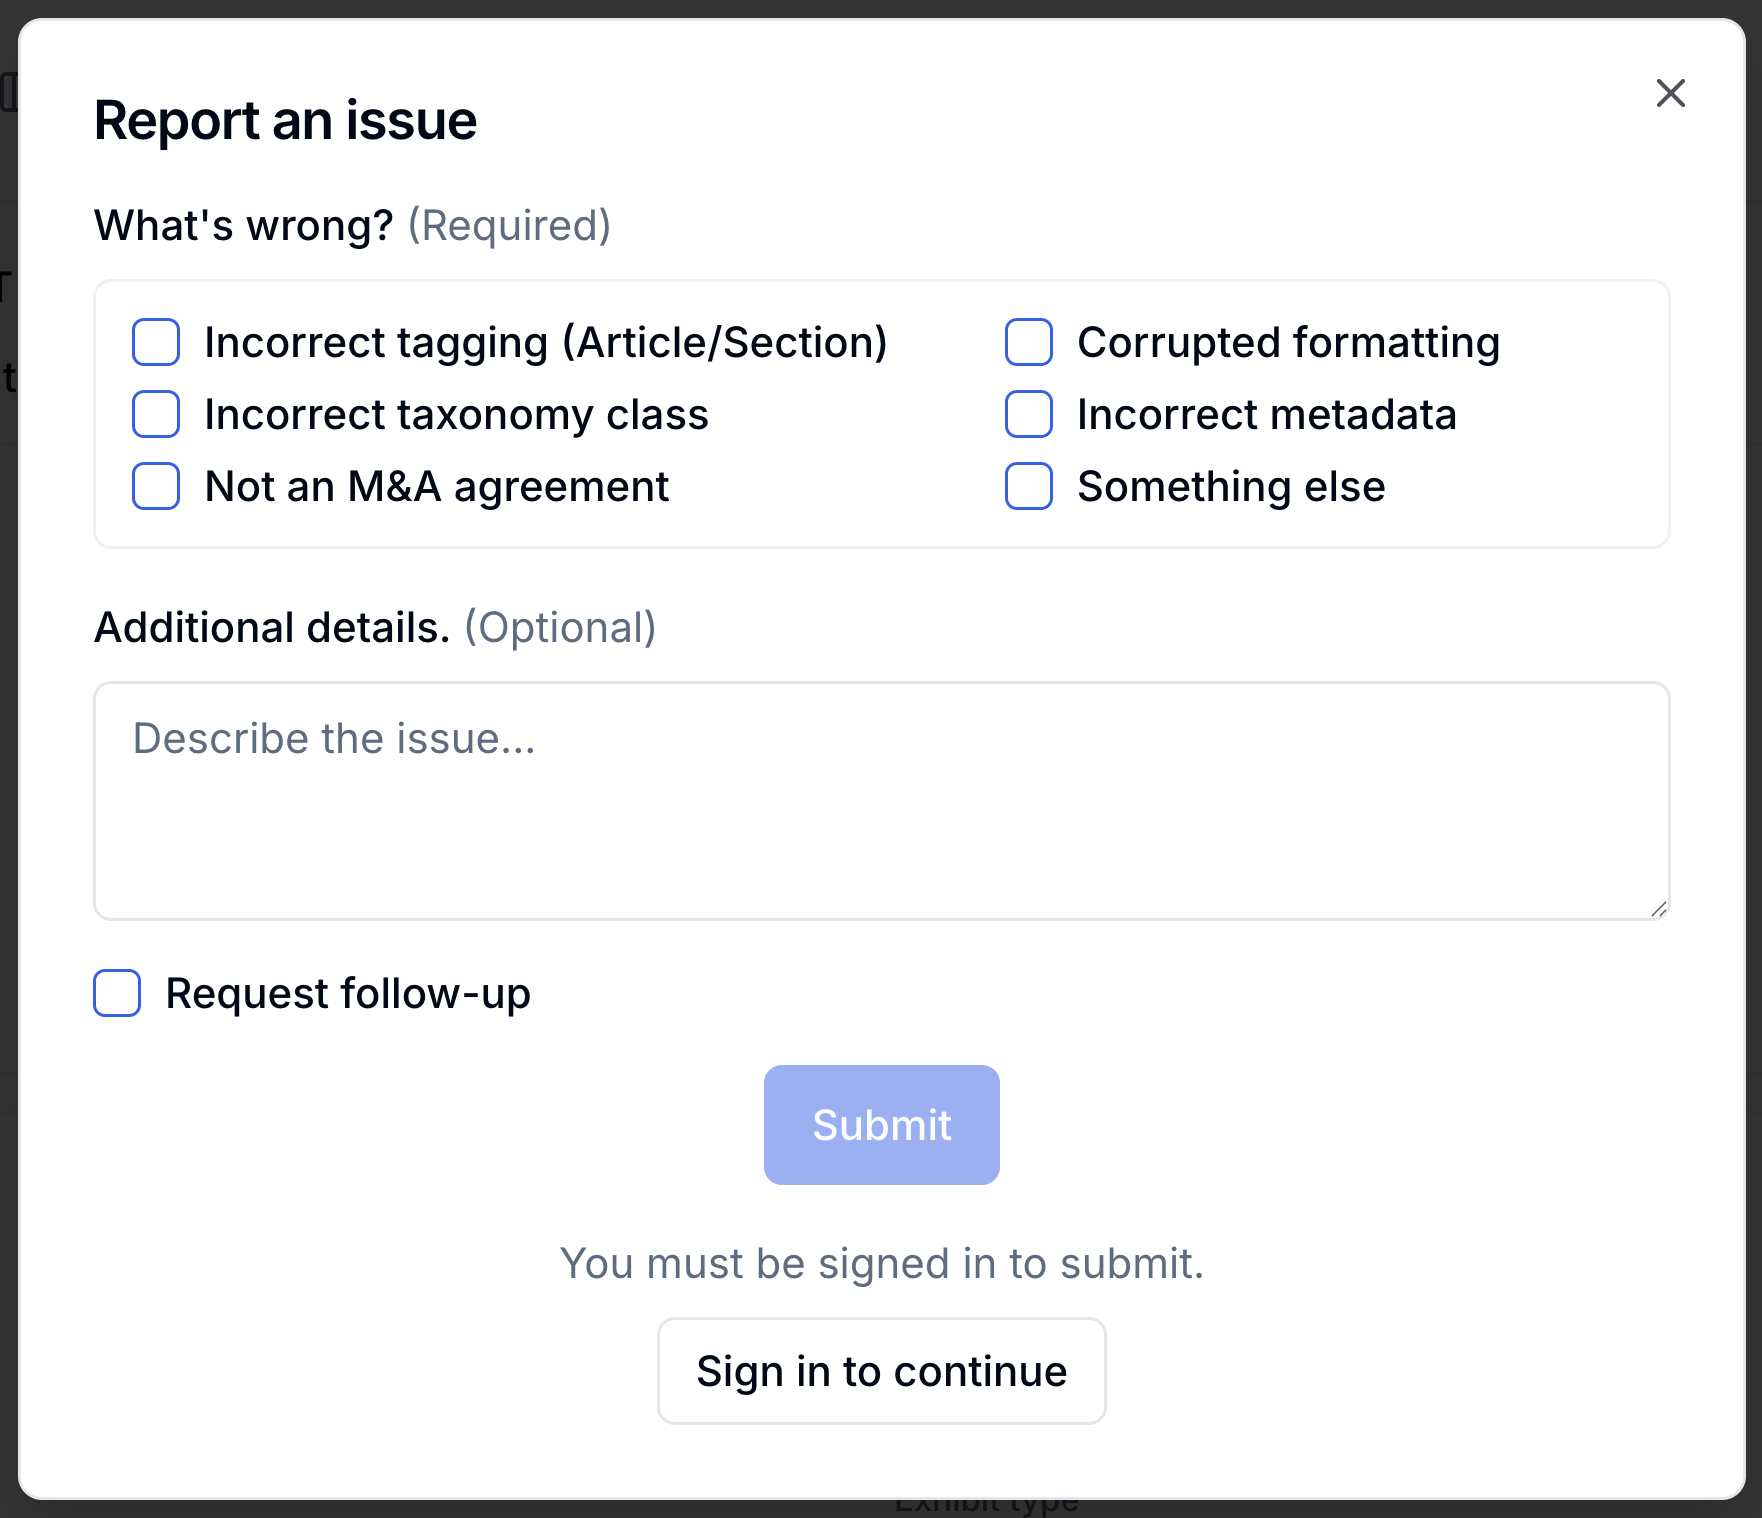
\includegraphics[width=0.9\textwidth,height=0.7\textheight,keepaspectratio]{report_issue.png}

\small \textbf{Example.} Interface for reporting data issues from the hosted site, as of 4/28/2026.
\end{center}

\end{appendices}

\end{document}
